\documentclass{article}

\usepackage{ctex}%提供中文
\usepackage{enumerate}%提供enumerate标号指定,如\begin{enumerate}[(1)],不过本文没用
\usepackage{amsmath}%数学包必有
\usepackage{amsfonts}%一些特殊的数学字体
\usepackage{amssymb}%特殊数学符号,如\therefore,amsmath不提供这些符号
\usepackage{amsthm}%定制定理环境,不过本文没用到
\usepackage{upgreek}%提供希腊字母直立体,如\uppi(国标里圆周率pi需要直立)
\usepackage{extarrows}%特殊的箭头和等号,提供\xlongequal,\xrightarrow等命令,可以在等号和箭头上加文字
\usepackage{bm}%提供命令\bm{P},用于数学环境加粗,以替代\boldsymbol{P}
\usepackage{url}%提供\url{}命令,防止有些url里面会有下划线_,这样会报错没有使用$$数学环境
\usepackage{float}%浮动体包,以figure浮动体为例,提供\begin{figure}[H],H参数表示强制将浮动体放在此处,禁止浮动
\usepackage{enumitem}%提供特殊标号,如\begin{enumerate}[label=(\roman*)],或者[label=(\chinese*)]或[label=(\alph*)]等,比enumerate包更自由
\usepackage{color}%提供颜色
\usepackage{geometry}%定制页面布局
\usepackage{framed}%提供定制framed环境,如23,24行定制的problem环境
\usepackage{tikz}%画图包
\usetikzlibrary{arrows.meta}%提供tikz特殊箭头
\usetikzlibrary{positioning}%提供TikZ各node的相对位置
\usetikzlibrary{decorations.pathreplacing}%提供大括号显示某段距离
\usepackage{hyperref}%提供超链接,hyperref包一定要放在最后引用,因为它大量renewcommand了一些命令

\geometry{
  textwidth=140mm,
  textheight=220mm,
  left=27mm,
  right=27mm,
  top=25.4mm, 
  bottom=25.4mm,
  headheight=2cm,
  headsep=4mm,
  footskip=12mm,
  heightrounded,
}
\newenvironment{problem}[1]{\begin{framed}\par\noindent\textbf{#1} }{\end{framed}\par}
\newenvironment{solution}[1][]{\noindent\textcolor{green}{Solution} \textcolor{red}{#1}\\ }%这里的参数指的是解法1或解法2

\newcommand{\e}{\mathrm{e}}
\newcommand{\E}{\mathbb{E}}
\newcommand{\var}{\mathrm{Var}}
\newcommand{\cov}{\mathrm{Cov}}
\renewcommand{\d}{\,\mathrm{d}}
\newcommand{\p}{\mathbb{P}}
\newcommand{\iid}{\,\mathrm{i.i.d.}\,}
\newcommand{\poi}{\text{Poi}\,}
\newcommand{\Exp}{\text{Exp}\,}
\newcommand{\res}{\text{Res}}

\title{方兆本随机过程第三版答案整理}
\author{ypa}
\date{2022.12.19\\ Last Modified: \today}

\begin{document}
\maketitle

\setcounter{section}{-1}
\section{前言}
尚未完成的题目:
\begin{enumerate}[label=(\chinese*)]
	\item 1.11
	\item 2.5
	\item 3.25-3.31
	\item 4.9 4.18 4.19 4.30 4.32 4.33 4.35-4.42
\end{enumerate}
第三章Markov过程中纯生过程、生灭过程、分支过程不讲;第四章平稳过程中白噪声序列、AR($p$)模型、Yule-Walker方程等不讲

\tableofcontents

\clearpage
\section{第一章~引论}
\begin{problem}{1.1}
    令$X(t)$为二阶矩存在的随机过程. 试证它是宽平稳的当且仅当$\E[X(t)]$与$\E[X(t)X(s+t)]$都不依赖$s$.
\end{problem}
\begin{solution}
    \textcolor{blue}{充分性:}\\
    若$\E[X(s)]$与$\E[X(s)X(s+s')]$都不依赖$s$\\
    则$\E[X(s)] = $ 常数$m$, $\E[X(s)X(s+s')] = f(t)$\\
    令$s' = s + t$,\\
    \[\therefore \E[X(s)X(s')] = f(s'-s)\]
    \[
        \begin{aligned}
        \therefore R_X(s, s')  & = \E[X(s)X(s')] - \E[X(s)]\E[X(s')] \\
        & = f(t - s) - m^2
        \end{aligned}
    \]
    $\therefore X(t)$是宽平稳的\\
    \textcolor{blue}{必要性:}\\
    若$X(t)$宽平稳则$\E[X(S)]$为常数$m$, 即$\E[X(S)]$与$s$无关\\
	则
    \[
        \begin{aligned}
         R_X(s, s') & = \E[X(s)X(s')] - \E[X(s)]\E[X(s')] \\
        & = g(s' - s) \\
        \end{aligned}
    \]
    令$s' = s + t$ \\
    则$\E[X(s)X(s+t)] = m^2 + g(t)$与$s$无关\\
\end{solution}

\begin{problem}{1.2}
    记$U_1, \cdots, U_n$为在$(0,1)$中均匀分布的独立随机变量. 对$0<t,x<1$定义
    \[ I(t,x) =
		\begin{cases}
		1, & \text{ $x \leqslant t$,} \\
		0, & \text{ $x > t$,}
		\end{cases}
	\]
    并记$\displaystyle X(t) = \frac{1}{n}\sum^n_{k=1}I(t,U_k), 0 \leqslant t \leqslant 1, $这是$U_1, \cdots, U_n$的经验分布函数. 试求过程$X(t)$的均值和协方差函数.
\end{problem}
\begin{solution}
    \[\E[X(t)] = \E\left[\frac{1}{n}\sum^n_{k=1}I(t, U_k)\right] = \E[I(t, U_1)] = \int^t_0 1 \d x = t\]
	\[\begin{aligned}
	R_X(s, t) & = \E [X(s)X(t)] - \E[X(s)\E X(t)]\\
			& = \E\left[\frac{1}{n^2}\sum_{i=1}^n I(s, U_i) \cdot \sum_{j=1}^n I(s, U_j)\right] - st\\
			& = \frac{1}{n^2}\Big\{(n^2 - n)\E[I(s, U_1) \cdot I(t, U_2)] + n\E[I(s, U_1) \cdot I(t, U_1)]\Big\} - st\\
			& = \frac{1}{n^2}[(n^2 - n)st + n \cdot \min(s, t)] - st\\
			& = \frac{1}{n}[\min(s, t) - st]
	\end{aligned}\]
\end{solution}

\begin{problem}{1.3}
    令$Z_1, Z_2$为独立的正态随机变量,均值为$0$,方差为$\sigma^2$,~$\lambda$为实数.定义过程$X(t) = Z_1\cos\lambda t + Z_2\sin\lambda t$.试求$X(t)$的均值函数和协方差函数.它是宽平稳的吗?
\end{problem}
\begin{solution}
    \[\begin{aligned}
	\E[X(t)] & = \E(Z_1)\cos \lambda t + \E(Z_2)\sin\lambda t = 0\\
	R_X(s, t) & = \cov[(Z_1\cos\lambda s + Z_2\sin\lambda s), (Z_z\cos\lambda t + Z_2\sin\lambda t)]\\
			& = \cov(Z_1, Z_1)\cos\lambda s \cos\lambda t + \cov(Z_2, Z_2)\sin\lambda s \sin\lambda t\\
			& = \sigma^2\cos\lambda(s - t)\\
	\end{aligned}\]
	$R_X(s,t)$只与$s-t$有关,故是宽平稳的
\end{solution}

\begin{problem}{1.4}
    Poisson过程$X(t), t \geqslant 0 $满足
    \begin{enumerate}[label=(\roman*)]
        \item $X(t) = 0$
        \item 对$t > s$,~$X(t) - X(s)$~服从均值为$\lambda (t-s)$的Possion分布
        \item 过程是有独立增量的.~
    \end{enumerate}
    试求其均值函数和协方差函数.它是宽平稳的吗?
\end{problem}
\begin{solution}
    \[\begin{aligned}
	\E[X(t)] & = \E [X(t) - X(0)] = \lambda t\\
	R_X(s, t) & = \cov[X(t), X(s)]\\
			& = \cov\left[\big(X(s) - X(t) + X(t) - X(0)\big), \big(X(t) - X(0)\big)\right]\\
			& = \cov(X(t) - X(0), X(t) - X(0)) \quad \text{(独立增量)}\\
			& = \lambda t \quad (s \geqslant t)
	\end{aligned}\]
	故非宽平稳
\end{solution}

\begin{problem}{1.5}
    $X(t)$为第4题中的Possion过程. 记$Y(t) = X(t+1) - X(t)$, 试求过程$Y(t)$的均值函数和协方差函数, 并研究其平稳性.
\end{problem}
\begin{solution}
    \[\begin{aligned}
	\E[Y(t)] & = \E[X(t+1)] - \E[X(t)] = \lambda\\
	R_X(s, t) & = \cov(X(s+1) - X(s), X(t+1) - X(t))\\
			& = \cov(X(s+1), X(t+1)) + \cov(X(s), X(t))\\
			& \qquad - \cov(X(s), X(t+1)) - \cov(X(s+1), X(t))\\
			& = \lambda [\min (s+1, t+1) + \min (s, t) - \min (s, t+1) - \min (s+1, t)]\\
	\end{aligned}\]
	令$\beta = s - t$, 当$\beta > 1$或$\beta < -1$时, $R_Y(s, t) = 0$ \\
	当$0 < \beta \leqslant 1$时, $R_Y(s, t) = \lambda (t + 1 + t - s - t) = \lambda (t - s + 1)$\\
	当$-1 \leqslant \beta \leqslant 0$时, $R_Y(s, t) = \lambda (s + 1 + s - s - t) = \lambda (s - t + 1)$\\
	故为宽平稳
\end{solution}

\begin{problem}{1.6}
    令$ Z_1 $和$ Z_2 $是独立同分布的随机变量. $\p(Z_1 = -1) = \p(Z_1 = 1) = \frac{1}{2}$. 记$X(t) = Z_1\cos\lambda t + Z_2\sin\lambda t$, $t \in \mathbb{R}$. 试证$X(t)$是宽平稳的, 它是严平稳的吗?
\end{problem}
\begin{solution}
    \[\begin{aligned}
		\E(Z_1) & = \E(Z_2) = 0\\
		\E[X(t)] & = \E(Z_1)\cos\lambda t + \E(Z_2)\sin\lambda t = 0\\
		R_X(s, t) & = \cov[(Z_1\cos\lambda s + Z_2\sin\lambda s), (Z_1\cos\lambda t + Z_2\sin\lambda t)]\\
			& = \cov(Z_1, Z_1)\cos\lambda s \cos\lambda t + \cov(Z_2, Z_2)\sin\lambda s\sin\lambda t\\
			& = 2 \var(Z_1)\cos\lambda(s-t)\\
			& = 2\left[\E (Z_1^2) - \E ^2(Z_1)\right]\cos\lambda(s-t)\\
			& = \cos\lambda(s-t)
	\end{aligned}\]
	故是宽平稳\\
	$F_t(x) = \p(Z_1\cos\lambda t + Z_2\sin\lambda t \leqslant x)$\\
	考虑$F_t(0) = \p(Z_1\cos\lambda t + Z_2\sin\lambda t \leqslant 0)$\\
	当$t = 0$时 $F_t(0) = \p(Z_1 \leqslant 0) = \frac{1}{2}$\\
	当$t = \frac{\uppi}{4\lambda}$时 $F_t(0) = \p\left(\frac{\sqrt{2}}{2}(Z_1+Z_2) \leqslant 0\right) = \frac{3}{4}$\\
	$\therefore F_t(x)$与$t$有关, 故$X(t)$不是严平稳过程
\end{solution}

\begin{problem}{1.7}
	试证:若$Z_0, Z_1,\cdots $为独立同分布随机变量, 定义$ X_n = Z_0 + Z_1 + \cdots + Z_n$, 则$\{X_n, n \geqslant 0\}$ 是独立增量过程.
\end{problem}
\begin{solution}
	对$\forall n$及$\forall t_1, \cdots, t_n\in \{0,1,2,\cdots\}, t_1 < t_2 < \cdots < t_n$, 有
	\[\begin{cases}
		X(t_2) - X(t_1) = Z_{t_1+1}+\cdots+Z_{t_2},\\
		X(t_3) - X(t_2) = Z_{t_2+1}+\cdots+Z_{t_3},\\
		\quad \vdots \\
		X(t_n) - X(t_{n-1}) = Z_{t_{n-1}+1}+\cdots+Z_{t_n}.\\
	\end{cases}\]
	由题知$Z_{t_1+1}, \cdots, Z_{t_n}$互相独立,\\
	$\therefore(Z_{t_1+1},\cdots,Z_{t_2}),(Z_{t_2+1},\cdots,Z_{t_3}),\cdots,(Z_{t_{n\!-\!1}\!+\!1},\cdots,Z_{t_n})$互相独立,\\
	$\therefore \{X_n, n \geqslant 0\}$为独立增量过程.
\end{solution}

\begin{problem}{1.8}
	若$X_1, X_2,\cdots $为独立随机变量, 还要添加什么条件才能确保它是严平稳的随机过程?
\end{problem}
\begin{solution}
	若$\{X_1, X_2, \cdots \}$严平稳, 则对任意正整数$m$和$n$, $X_m$和$X_n$的分布都相同, 从而$X_1, X_2, \cdots $是一列同分布的随机变量. 而当$X_1, X_2, \cdots $是一列独立同分布的随机变量时. 对任意正整数$k$及$n_1, \cdots,n_k, k$维随机向量$\left(X_{n_1}, \cdots, X_{n_k}\right)$的分布函数为(记$X_1, X_2, \cdots $的共同分布函数为$F(x)$)\\
	\[\begin{split}
	& F_{X_{n_1}, \cdots, X_{n_k}}(x_1, \cdots, x_k)  = F_{X_{n_1}}(x_1)\cdots F_{X_{n_k}}(x_n)\\
		 = & F(x_1)\cdots F(x_k).\qquad (-\infty < x_1,\cdots,x_k < +\infty)\\
	\end{split}\]
	这说明了$(X_{n_1},\cdots,X_{n_k})$的分布函数与$n_1, \cdots, n_k$无关, 故$\{X_1, X_2, \cdots\}$严平稳.\\
\end{solution}

\begin{problem}{1.9}
	令$X$和$Y$是从单位圆内的均匀分布中随机选取一点所得的横坐标和纵坐标. 试计算条件概率
	\[\p\left(X^2+Y^2 \geqslant \frac{3}{4} \bigg| X > Y\right).\]
\end{problem}
\begin{solution}
	\begin{minipage}[c]{0.3\textwidth}
		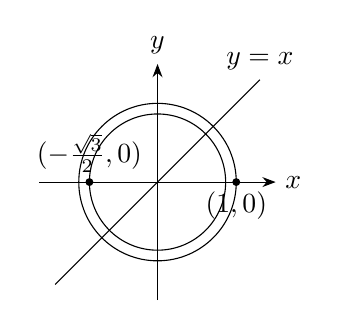
\begin{tikzpicture}[>=Stealth]
			\draw [->] (-1.5,0) -- (1.5,0) node[right] {$x$};
			\draw [->] (0,-1.5) -- (0,1.5) node[above] {$y$};
			\draw (1,0)arc(0:360:1) (0.865,0)arc(0:360:0.865);
			\draw (1,0)node[below]{$(1,0)$};
			\draw (-0.865,0)node[above]{$(-\frac{\sqrt{3}}{2},0)$};
			\fill (1,0)circle(0.05) (-0.865,0)circle(0.05);
			\draw (-1.3,-1.3)--(1.3,1.3)node[above]{$y=x$};
		\end{tikzpicture}	
	\end{minipage}
	\begin{minipage}[c]{0.65\textwidth}
		由对称性得,
		\[\begin{aligned}
			&\p\left(X^2+Y^2 \geqslant \frac{3}{4} \bigg| X > Y\right)\\
			=& \frac{1}{2}\cdot \p\left(X^2+Y^2 \geqslant \frac{3}{4} \right)\\
			=&\frac{1}{2}\cdot (1-\frac{3}{4})=\frac{1}8\\
		\end{aligned}\]
	\end{minipage}
\end{solution}

\begin{problem}{1.10}
	粒子依参数为$\lambda $的Possion分布进入计数器, 两粒子到达的时间间隔$T_1, T_2,\cdots $是独立的参数为$\lambda $的指数分布随机变量. 记$S$是$[0,1]$时段中的粒子总数. 时间区间$I\subset [0,1]$, 其长度记为$|I|$. 试证明$\p(T_1\in I, S = 1) = \p(T_1\in I, T_1 + T_2 > 1)$, 并由此计算$\p(T_1\in I|S = 1) = |I|$.
\end{problem}
\begin{solution}
	设$W_i$为第$i$个离子进入计数器时的时刻,显然有$W_n =\sum_{k=1}^{n}T_k$
	那么有$\{S=1\}=\{W_2>1\}\Rightarrow \{T_1\in I,S=1\}=\{S=1\}=\{T_1\in I,T_1+T_2>1\}$
	于是有\[\p(T_1\in I,S=1)=\p(T_1\in I,T_1+T_2>1)\]
	\[\begin{aligned}
		\p(T_1\in I|S=1) & = \frac{\p(T_1\in I,S=1)}{\p(S=1)}\\
		& = \frac{\p[N(t)=0, N(t+|I|=1,N(1)=1)]}{\p[N(1)=1]}\\
		& = \frac{\e^{-\lambda t}\cdot \lambda |I|\cdot \e^{-\lambda |x|}\cdot \e^{-\lambda (1-t-|I|)}}{\lambda \e^{-\lambda}}\\
		& = |I|
	\end{aligned}\]
\end{solution}

\begin{problem}{1.11}
	$X, Y$为两独立随机变量且分布相同. 证明$\E (X|X+Y = z) = \E (Y|X+Y = z)$. 并试求基于$X+Y=z$的$X$的最佳预报, 并求出预报误差$\E (X-\phi (X+Y))^2$
\end{problem}
\begin{solution}
	本题暂缺
\end{solution}

\begin{problem}{1.12}
	气体分子的速度$V$有三个垂直分量$V_x, V_y, V_z$, 它们的联合分布密度依Maxwell-Boltzman定律为
	\[f_{V_x, V_y, V_z}(v_1, v_2, v_3) = \frac{1}{(2\uppi kT)^{3/2}}\exp\left\{-\left(\frac{v^2_1+v^2_2+v^2_3}{2kT}\right)\right\},\]
	其中$k$是Boltzman常数, $T$为绝对温度, 给定分子的总动能为$e$. 试求$x$方向的动量的绝对值的期望值.
\end{problem}
\begin{solution}
	\[\begin{aligned}
		f_{V_x,V_y,V_z}(v_x,v_y,v_z) & = \frac{1}{(2\uppi kT)^{3/2}}\exp\left\{-\frac{v_x^2 + v_y^2 + v_z^2}{2kT}\right\}=\frac{\e^{-\frac{v_x^2}{2kT}}}{\sqrt{2\uppi}\sqrt{kT}}\cdot \frac{\e^{-\frac{v_y^2}{2kT}}}{\sqrt{2\uppi}\sqrt{kT}}\cdot \frac{\e^{-\frac{v_z^2}{2kT}}}{\sqrt{2\uppi}\sqrt{kT}}\\
		V_x,V_y,V_z & \sim N(0,kT)\\
		e & = \E\left[\frac{1}{2}mV^2\right]=\frac{1}{2}m\E[V^2]=\frac{1}{2}m\E[V_x^2+V_y^2+V_z]=\frac{1}{2}m\cdot 3kT=\frac{3mkT}{2}\\
		m & = \frac{2e}{3kT}\\
		\E[\left|p_x\right|] & = m\E[\left|v_x\right|]=m \int_{-\infty}^{+\infty}\frac{1}{\sqrt{2\uppi}\sqrt{kT}}\left|v_x\right|\e^{-\frac{v_x^2}{2kT}}\d v_x\\
		& = \frac{2m}{(2\uppi kT)^{\frac{1}{2}}}\int_{0}^{+\infty}v_x \e^{-\frac{v_x^2}{2kT}}\d v_x\\
		& = m\sqrt{\frac{2kT}{\uppi}} = \frac{2e}{3kT}\sqrt{\frac{2kT}{\uppi}} = \frac{2e}{3}\sqrt{\frac{2}{\uppi kT}}\\
	\end{aligned}\]
\end{solution}

\begin{problem}{1.13}
	若$X_1, X_2,\cdots, X_n$独立同分布. 它们服从参数为$\lambda$的指数分布. 试证$\sum\limits^n_{i=1}X_i$是参数为$(n, \lambda)$的$\Gamma$分布, 其密度为
	\[f(t) = \lambda \exp\{-\lambda t\}(\lambda t)^{n-1}/(n-1)!\, ,\quad t \geqslant 0.\]
\end{problem}
\begin{solution}
	$X_i$的矩母函数为\[g_{X_i}(t)=\int_{0}^{+\infty}\lambda \e^{-\lambda x}\cdot \e^{tx}\d x = \frac{\lambda}{\lambda -t}\]
	\[\because X_1,X_2,\dots ,X_n \iid \quad \therefore g_{X_1,X_2,\dots ,X_n}(t) = \left(g_{X_i}(t)\right)^n = \left(\frac{\lambda}{\lambda - t}\right)^n\]
	参数为$(n, \lambda )$的$\Gamma $分布的矩母函数为:
	\[\begin{aligned}
		g_{\Gamma }(t) & = \int_{0}^{+\infty}\frac{\lambda \e^{-\lambda x}(\lambda x)^{n-1}}{(n-1)!}\cdot \e^{tx}\d x\\
		& = \frac{\lambda ^n}{(n-1)!}\int_{0}^{+\infty}x^{n-1}\e^{-(\lambda -t)x}\d x \\
		& \xlongequal{u=(\lambda -t)x} \frac{\lambda ^n}{(n-1)!}\int_{0}^{+\infty}\frac{u^{n-1}\e^{-u}}{(\lambda -t)^n}\d u \\
		& = \frac{\lambda ^n}{(n-1)!}\cdot \frac{1}{(\lambda -t)^n}\cdot \Gamma(n)\\
		& = \frac{\lambda ^n}{(n-1)!}\cdot \frac{1}{(\lambda -t)^n}\cdot (n-1)! = \left(\frac{\lambda}{\lambda -t}\right)^n\\
	\end{aligned}\]
	$\sum_{i=1}^{n}X_i$是参数为$(n,\Gamma )$的$\Gamma $分布
\end{solution}

\begin{problem}{1.14}
	设$X_1$和$X_2$为相互独立的均值为${\lambda}_1$和${\lambda}_2$的Possion随机变量. 试求$X_1+X_2$的分布, 并计算给定$X_1+X_2 = n$时$X_1$的条件分布.
\end{problem}
\begin{solution}
	令$Y = X_1+X_2$
	\[\begin{aligned}
	g_Y(t) & = g_{X_1}(t)g_{X_2}(t)\\
			& = \e^{{\lambda}_1(\e^t-1)}\e^{{\lambda}_2(\e^t-1)}\\
			& = \e^{({\lambda}_1 + {\lambda}_2)(\e^t-1)}
	\end{aligned}\]
	$\therefore Y \sim \poi({\lambda}_1+{\lambda}_2)$\\
	$\therefore $给定$X_1+X_2 = n$时$X_1$服从参数为$p = \frac{{\lambda}_1}{{\lambda}_1 + {\lambda}_2}, n = n$的二项分布
	\[\begin{aligned}
		\p[X_1+X_2=n] & = \frac{\e^{-(\lambda_1+\lambda_2)}(\lambda_1+\lambda_2)^n}{n!}\\
		\p[X_1=m|X_1+X_2=n] & = \frac{\p[X_1=m,X_1+X_2=n]}{\p[X_1+X_2=n]}=\frac{\p[X_1=m,X_2=n-m]}{\p[X_1+X_2=n]}\\
		& = \frac{\frac{\e^{-\lambda_1}\lambda_1^m}{m!}\cdot \frac{\e^{-\lambda_2}\lambda_2^{n-m}}{(n-m)!}}{\frac{\e^{-(\lambda_1+\lambda_2)}(\lambda_1+\lambda_2)^n}{n!}}\\
		& = \frac{\lambda_1 ^m \lambda_2 ^{n-m}n!}{m!(n-m)! \lambda_1 ^n \lambda_2 ^n}\\
		& = \binom{n}{m}\left(\frac{\lambda_1}{\lambda_1+\lambda_2}\right)^m \left(\frac{\lambda_2}{\lambda_1+\lambda_2}\right)^{n-m}
	\end{aligned}\]
	故服从二项分布
\end{solution}

\begin{problem}{1.15}
	若$X_1, X_2,\cdots $独立且有相同的以$\lambda$为参数的指数分布, $N$服从几何分布, 即
	\[\p(N = n) = \beta(1-\beta)^{n-1}, n = 1,2,\cdots, 0<\beta<1.\]
试求随机和$\displaystyle Y = \sum_{i=1}^N X_i$的分布.
\end{problem}
\begin{solution}[1]
	\[\E(\e^{tY}|N = n) = g^n_X (t) = \left(\frac{\lambda}{\lambda - t}\right)^n \overset{\Delta}{=} {\alpha}^n\]
	\[\therefore g_Y(t) = \E[\E(\e^{tY}|N)] = \E({\alpha}^N) = \sum^{+\infty}_{n=1}\beta(1-\beta)^{n-1}{\alpha}^n = \sum^{+\infty}_{n=1}\alpha\beta(\alpha-\alpha\beta)^{n-1}\]
	当$|\alpha -\alpha\beta|<1$时$g_Y(t)=\frac{\alpha\beta}{1-\alpha(1-\beta)} = \frac{\lambda\beta}{\lambda\beta - t}$\\
	$\therefore Y$服从参数为$\lambda\beta$的指数分布
\end{solution}
\begin{solution}[2]
	利用题1.13的结论
	\[X_1,\dots ,X_n \iid \quad X_i\sim \Exp(\lambda ) \Rightarrow f(t)=\frac{\lambda \e^{-\lambda t}(\lambda t)^{n-1}}{(n-1)!}\]
	\[\begin{aligned}
		f_Y(y) & = \sum_{n=1}^{\infty}f_{Y|N}(y|n)\p[N=n]=\sum_{n=1}^{\infty}\frac{\lambda ^n\e^{-\lambda t}t^{n-1}}{(n-1)!}\beta(1-\beta)^{n-1}\\
		& = \beta \e^{-\lambda t}\sum_{n=1}^{\infty}\frac{\lambda ^n\left[(1-\beta)t\right]^{n-1}}{(n-1)!}\\
		& = \lambda \beta \e^{-\lambda t}\sum_{n=1}^{\infty}\frac{(\lambda t(1-\beta ))^{n-1}}{(n-1)!}\\
		& = \lambda \beta \e^{-\lambda t}\cdot \e^{\lambda t(1-\beta)} = \lambda \beta \e^{-\lambda \beta t}
	\end{aligned}\]
\end{solution}

\begin{problem}{1.16}
	若$X_1, X_2, \cdots$独立同分布, $P(X_i = \pm 1) = \frac{1}{2}$. $N$与$X_i$, $i \geqslant 1$独立且服从参数为$\beta$的几何分布, $0 < \beta < 1$. 试求随机和$Y = \sum\limits^N_{i=1} X_i$的均值, 方差和三、四阶矩.
\end{problem}
\begin{solution}[1]
	使用矩母函数法。但据助教的习题提示,没有使用MATLAB等软件,矩母函数法求出来的应该是错误的\cite{郑班助教}
	\[\E(\e^{tY}|N = n) = g^n_X (t) = \E^n(\e^{tY}) = {\left(\frac{\e^t + \e^{-t}}{2}\right)}^n\]
	\[\therefore g_Y(t) = \E\left[\E(\e^{tY}|N)\right] = \E\left[\left(\frac{\e^t + \e^{-t}}{2}\right)^N\,\right] = \sum^{\infty}_{n=1}\left(\frac{\e^t + \e^{-t}}{2}\right)^n \beta (1 - \beta)^{n - 1}\]
	\[\begin{aligned}
	\therefore \E(Y) & = g'_Y(0) = \sum^{\infty}_{n=1} n \left(\frac{\e^t + \e^{-t}}{2}\right)^{n - 1}\beta (1 - \beta)^{n - 1} \frac{\e^t - \e^{-t}}{2} \bigg|_{t=0} = 0 \\
	\E(Y^2) & = g''_Y(0) = \sum^{\infty}_{n=1}\bigg[ n(n-1)\left(\frac{\e^t + \e^{-t}}{2}\right)^{n-2}\beta (1 - \beta)^{n - 1} \left(\frac{\e^t - \e^{-t}}{2}\right)^2 + \\
		& \qquad n\left(\frac{\e^t + \e^{-t}}{2}\right)^n\beta (1 - \beta)^{n - 1} \bigg] \Bigg|_{t=0} = \sum^{\infty}_{n=1}n\beta(1-\beta)^{n-1} = \frac{1}{\beta}\\
	\var(Y) & = \E(Y^2)-\E^2(Y) = \frac{1}{{\beta}^2}\\
	\E(Y^3) & = g^{(3)}_Y(0)\\
		& = \left(\sum^{\infty}_{n=1}\left\{n\beta(1-\beta)^{n-1}\left[(n-1)\left(\frac{\e^t+\e^{-t}}{2}\right)^{n-2}{\frac{\e^t-\e^{-t}}{2}}^2+\left(\frac{\e^t+\e^{-t}}{2}\right)^n\right]\right\}\right)'\Bigg|_{t=0}\\
		& = \sum^{\infty}_{n=1}\Bigg\{ n\beta{(1-\beta)}^{n-1}\Bigg[(n-1)(n-2)\left(\frac{\e^t+\e^{-t}}{2}\right)^{n-2}\left(\frac{\e^t-\e^{-t}}{2}\right)^{3}+ \\
		& \qquad (n-1)\left(\frac{\e^t+\e^{-t}}{2}\right)^{n-2} \cdot 2 \cdot \frac{\e^t-\e^{-t}}{2} \cdot \frac{\e^t+\e^{-t}}{2} + n \cdot \left(\frac{\e^t+\e^{-t}}{2}\right)^{n-1} \cdot \frac{\e^t-\e^{-t}}{2} \Bigg] \Bigg\} \Bigg|_{t=0}\\
		& = 0 \\
    \E(Y^4) & = g^{(4)}_Y(0)\\
        & = \sum^{\infty}_{n=1}\left\{n\beta(1-\beta)^{n-1}\left[(n-1)\left(\frac{\e^t+\e^{-t}}{2}\right)^{n-1}(\e^t+\e^{-t})+n\left(\frac{\e^t+\e^{-t}}{2}\right)^{n}\right]\right\} \Bigg|_{t=0}\\
        & = \sum^{\infty}_{n=1}(3n^2-2n)\beta(1-\beta)^{n-1} = 3\sum^{\infty}_{n=1}n^2\beta(1-\beta)^{n-1} - 2\sum^{+\infty}_{n=1}n\beta(1-\beta)^{n-1}\\
        & = 3\left(\frac{1-\beta}{{\beta}^2} + \frac{1}{{\beta}^2}\right) - 2\frac{1}{{\beta}^2} = \frac{6-5\beta}{{\beta}^2}
	\end{aligned}\]
\end{solution}
\begin{solution}[2]
	使用条件期望
	\[\begin{aligned}
		\E(Y|N=n) & = \E\left(\left.\sum_{i=1}^{N}X_i\right|N=n\right)=\E\left(\sum_{i=1}^{n}X_i\right) = n\E(X_i) =0\\
		\E(Y) & = \sum_{i=1}^{\infty}\E(Y|N=n)\p(N=n) = 0\\
		\E(Y^2|N=n) & = \E\left[\left.\left(\sum_{i=1}^{N}X_i\right)^2\right|N=n\right] = \E\left(\sum_{i=1}^{n}X_i^2+2\sum_{1\leqslant i<j\leqslant n}X_i X_j\right)\\
		& = n\E(X_i^2)+2\sum \E(X_i)\E(X_j) = n\\
		\E(Y^2) & = \sum_{i=1}^{\infty}\E(Y^2|N=n)\p(N=n) = \sum_{i=1}^{\infty}n\p(N=n) = \sum_{i=1}^{\infty}n\beta (1-\beta )^{n-1} = \frac{1}{\beta}\\
		\E(Y^3|N=n) & = \E\left(\sum_{i=1}^{n}X_i^3+3\sum_{1\leqslant i<j\leqslant n}X_i X_j^2+3\sum_{1\leqslant i<j\leqslant n}X_i^2 X_j\right)\\
		& = \E\left(\sum_{i=1}^{n}X_i^3 +3\sum_{i\neq j}X_i^2 X_j\right) = n\E(X_i^3) +3\sum_{i\neq j}\E(X_i^2)\E(X_j) = 0\\
		\E(Y^3) & = \sum_{i=1}^{\infty}\E(Y^3|N=n)\p(N=n) = 0\\
		\E(Y^4|N=n) & = \E\left(\sum_{i=1}^{n}X_i^4+4\sum_{1\leqslant i<j\leqslant n}X_i X_j^3+6\sum_{1\leqslant i<j\leqslant n}X_i^2 X_j^2+4\sum_{1\leqslant i<j\leqslant n}X_i^3 X_j\right)\\
		& = \E\left(\sum_{i=1}^{n}X_i^4 + 4\sum_{i\neq j}X_i^3 X_j + 6\sum_{i\neq j}X_i^2 X_j^2\right)\\
		& = n\E(X_i^4) + 0 + 6\cdot \binom{n}{2}\E(X_i^2 X_j^2) = n + 6\cdot \binom{n}{2} = 3n^2 - 2n\\
		\E(Y^4) & = \sum_{i=1}^{\infty}\E(Y^4|N=n)\p(N=n) = \sum_{i=1}^{\infty}3n^2\beta (1-\beta )^{n-1} - 2\sum_{i=1}^{\infty}n\beta (1-\beta )^{n-1}\\
		& = \frac{6-5\beta}{{\beta}^2}
	\end{aligned}\]
	计算$\E(Y^4)$时会出现一项$\sum_{i=1}^{\infty}n^2\beta (1-\beta )^{n-1}$,计算方法如下:
	\[\begin{aligned}
		\sum_{i=1}^{\infty}n^2\beta (1-\beta )^{n-1} & = \beta \sum_{i=1}^{\infty}[n(n-1)+n](1-\beta )^{n-1}\\
		& = \beta \left[\sum_{i=1}^{\infty}n(n-1)(1-\beta )^{n-1} + \sum_{i=1}^{\infty}n(1-\beta)^{n-1}\right]\\
		& = \beta \left[(1-\beta )\sum_{n=1}^{\infty}\left((1-\beta )^n\right)'' + \sum_{n=1}^{\infty}\left((1-\beta)^n\right)'\right]\\
		& = \beta \left[(1-\beta)\left(\frac{1}{\beta}-1\right)'' - \left(\frac{1}{\beta} - 1\right)'\right]\\
		& = \beta \left[\frac{2\beta(1-\beta)}{\beta ^3} + \frac{1}{\beta ^2}\right] = \frac{2-\beta}{\beta ^2}
	\end{aligned}\]
	或者可以采用稍微有点数学性的方法:
	$\E(Y^4) = \beta \sum_{n=1}^{\infty}n^2 (1-\beta)^{n-1}$在$(0,1)$上内闭一致收敛,$\therefore$求和和偏导次序可交换
	
	令$a = 1-\beta \Rightarrow n^2 a^{n-1}=\frac{\partial }{\partial a}(a\cdot \frac{\partial }{\partial a}a^n)$
	\[\begin{aligned}
		\sum_{n=1}^{\infty}n^2 a^{n-1} & = \sum_{n=1}^{\infty}\frac{\partial }{\partial a}\left(a \frac{\partial a^n}{\partial a}\right) = \frac{\partial }{\partial a}\left(a \frac{\partial \sum_{n=1}^{\infty}a^n}{\partial a}\right)\\
		& = \frac{\partial }{\partial a}\left(a \frac{\partial (\frac{a}{1-a})}{\partial a}\right) = \frac{1+a}{(1-a)^3} = \frac{2-\beta}{\beta ^3}
	\end{aligned}\]
\end{solution}

\begin{problem}{1.17}
	随机变量$N$服从参数为$\lambda$的Possion分布. 给定$N=n$, 随机变量$M$服从以$n$和$p$为参数的二项分布. 试求$M$的无条件概率分布.
\end{problem}
\begin{solution}
	\[
\begin{split}
& \E\big(\e^{tM}|N=n\big) = \big(p\e^t+(1-p)\big)^n \overset{\Delta}{=} a^n\\
& g_M(t) = \E(a^N) = \sum^{+\infty}_{n=0}a^n\frac{\lambda^n \e^{-\lambda}}{n!} = \e^{\lambda p(\e^t-1)}\\
& \therefore M \sim \poi(\lambda p)
\end{split}
\]
\end{solution}

\clearpage
\section{第二章 Poisson过程}
\begin{problem}{2.1}
	$N(t)$为一Possion过程, 对$s<t$试求条件概率$\p\{N(s) = k | N(t) = n\}$.
\end{problem}
\begin{solution}
	\[\begin{aligned}
		& \p\{N(s)=k|N(t)=n\} = \frac{\p[N(s)=k, N(t)=n]}{\p[N(t)=n]}\\
		= & \frac{\p[N(s)-N(0)=k, N(t)-N(s)=n-k]}{\p[N(t)=n]}\\ 
		= & \left[\frac{({\lambda s})^k\e^{-{\lambda s}}}{k!} \cdot \frac{\left(\lambda(t-s)\right)^{n-k} \e^{-\lambda(t-s)}}{(n-k)!}\right] \Bigg/ \left[\frac{(\lambda t)^n \e^{-\lambda t}}{n!}\right]\\
		= & \frac{n!}{k!(n-k)!}\left(\frac{s}{t}\right)^k \left(1-\frac{s}{t}\right)^{n-k}\\
	\end{aligned}\]
\end{solution}

\begin{problem}{2.2}
	$\{N(t), t \geqslant 0\}$为一强度是$\lambda$的Possion过程. 对$s > 0$试计算$E[N(t) \cdot N(t+s)]$.
\end{problem}
\begin{solution}
	\[\begin{aligned}
	\text{原式} & = \E[N(t)\textcolor{red}{(}N(t+s)-N(t)+N(t)\textcolor{red}{)}]\\
		& = \E[N(t)\textcolor{red}{(}N(t+s)-N(t)\textcolor{red}{)}]+\E[N^2(t)]\\
		& = \lambda t \cdot \lambda s + \var[N(t)] + \E^2[N(t)]\\
		& = \lambda ^2 ts+\lambda t + (\lambda t)^2\\
		& = \lambda ^2 t(s+t)+\lambda t
	\end{aligned}\]
\end{solution}

\begin{problem}{2.3}
	电报依平均速率为每小时3个的Possion过程到达电报局, 试问:
	\begin{enumerate}[label=(\roman*)]
		\item 从早上八时到中午没收到电报的概率;
		\item 下午第一份电报到达时间的分布是什么?
	\end{enumerate}
\end{problem}
\begin{solution}
	\begin{enumerate}[label=(\roman*)]
		\item 令$t$的计时单位为小时, 并以早上8:00为起始时刻,所求事件的概率即
		\[\p[N(4)=0]=\frac{\e^{-3\times 4} \cdot (3\times 4)^0}{0!} = \frac{1}{\e^{12}} \approx 6.1 \times 10^{-6}\]
		\item 取中午12:00为起始时刻, $T$表示下午第一份电报到达时间
		\[F(t) = \p(T \leqslant t) = \p[N(t) \geqslant 1] = 1 - \e^{-3t}\]
		$\displaystyle \therefore f(t) = \frac{\d F_T (t)}{\d t} = 3\e^{-3t}$, 即$T$服从参数为3的指数分布\\
	\end{enumerate}
\end{solution}

\begin{problem}{2.4}
	$\{N(t), t \geqslant 0\}$为一$\lambda = 2$的Possion过程, 试求:
	\begin{enumerate}[label=(\roman*)]
		\item $P\{N(1) \leqslant 2\}$;
		\item $P\{N(1) = 1 \text{\,且\,}N(2) = 3\}$;
		\item $P\{N(1) \geqslant 2 | N(1) \geqslant 1\}$.
	\end{enumerate}
\end{problem}
\begin{solution}
	\begin{enumerate}[label=(\roman*)]
		\item $\displaystyle \p[N(1)\leqslant 2] = \sum_{k=0}^{2}\p[N(1)=k]=\sum_{k=0}^{2}\frac{\e^{-2}2^k}{k!} = \frac{5}{\e^2}$
		\item $\displaystyle \text{原式} = \p[N(1)-N(0)=1]\p[N(2)-N(1)=2] = \frac{\e^{-2}2}{1!}\cdot \frac{\e^{-2} 2^2}{2!} = \frac{4}{\e^4}$
		\item \[\begin{aligned}
			\text{原式} & = \frac{\p[N(1) \geqslant 2 | N(1) \geqslant 1]}{\p[N(1) \geqslant 1]} = \frac{\p[N(1) \geqslant 2]}{\p[N(1) \geqslant 1]} = \frac{1-\p[N(1)-N(0) \leqslant 1]}{1-\p[N(1)-N(0)=0]}\\
						& = \frac{1-\frac{\e^{-2}2^0}{0!}-\frac{\e^{-2}2^1}{1!}}{1-\frac{\e^{-2}2^0}{0!}} = \frac{1-3\e^{-2}}{1-\e^{-2}} = \frac{\e^{2}-3}{\e^{2}-1}
			\end{aligned}\]
	\end{enumerate}
\end{solution}

\begin{problem}{2.5}
	证明概率$P_m(t) = \p[N(t) = m]$在命题2.1的假定$(1)\sim(4)$下满足微分方程
 	\[P'_m(t) = -\lambda P_m(t) + \lambda P_{m-1}(t),\quad m=1,2,\cdots, \]
 	并证明在初始条件下$P_m(0) = 0, m = 1,2,\cdots$下的解为$\displaystyle \frac{{\lambda}^m t^m}{m!}\e^{-\lambda t}$.
	\par 4个假定分别为:
	\begin{enumerate}[label=(\arabic*)]
		\item 在不相交区间中事件发生的数目相互独立,也即对任何整数$n=1,2,\cdots $,设时刻$t_0=0<t_1<t_2<\cdots <t_n$,增量$N(t_1)-N(t_0),N(t_2)-N(t_1),\cdots ,N(t_n)-N(t_{n-1})$相互独立;
		\item 对任何时刻$t$和正数$h$,随机变量(增量)$N(t+h)-N(t)$的分布只依赖于区间长度$h$而不依赖于时刻$t$;
		\item 存在正常数$\lambda $,当$h\downarrow 0$时,使在长度为$h$的小区间中事件至少发生一次的概率\[\p[N(t+h)-N(t)\geqslant 1]=\lambda h+o(h);\]
		\item 在小区间$(t,t+h]$发生两个或以上事件的概率为$o(h)$(可以忽略不计),即当$h\downarrow 0$,\[\p[N(t+h)-N(t)\geqslant 2]=o(h)\]
	\end{enumerate}
\end{problem}
\begin{solution}
	本题暂缺
\end{solution}

\begin{problem}{2.6}
	一部600页的著作总共有240个印刷错误, 试利用Possion过程近似求出某连续三页无错误的概率.
\end{problem}
\begin{solution}
	设Poisson参数为$\lambda $,有$600\lambda = 240 \Rightarrow \lambda = 0.4$
	\[\p[N(m+3)-N(m)=0]=\frac{\e^{-0.4\times 3}(0.4\times 3)^0}{0!} = \frac{1}{\e^{1.2}}\]
\end{solution}

\begin{problem}{2.7}
	$N(t)$是强度为$\lambda$的Possion过程. 给定$N(t) = n$, 试求第$r$个事件$(r \leqslant n)$发生的时刻$W_r$的条件概率密度$f_{W_r|N(t)=n}(w_r|n)$.
\end{problem}
\begin{solution}[1]
	\[\begin{aligned}
		& f_{W_r|N(t)=n}(w_r|n) \cdot \Delta w_r\\
		= & \p[N(w_r) - N(0) = r - 1, N(w_r+\Delta w_r)-N(w_r)=1|N(t) = n]\\
		= & \p[N(w_r) - N(0) = r - 1] \cdot \p[N(w_r+\Delta w_r)-N(w_r)=1]\\
		& \cdot \frac{\p[N(t)-N(w_r+\Delta w_r)=n-r]}{\p[N(t) = n]}\\
		= &\frac{\frac{(\lambda w_r)^{r-1}}{(r-1)!}\e^{-\lambda w_r} \cdot [\lambda \Delta w_r + o(\Delta w_r)] \cdot \frac{[\lambda (t-w_r-\Delta w_r)]^{n-r}}{(n-r)!} \e^{-\lambda(t-w_r-\Delta w_r)}}{\frac{(\lambda t)^n}{n!} \e^{\lambda t}}\\
		\end{aligned}\]
		两边除以$\Delta w_r$并令$\Delta w_r\to 0$得
		\[f_{W_r|N(t)=n}(w_r|n) = \frac{n!}{(r-1)!(n-r)!}\frac{(w_r)^{r-1}(t-w_r)^{n-r}}{t^n}\]
\end{solution}
\begin{solution}[2]
	直观理解如下
	\begin{figure}[H]
		\centering
		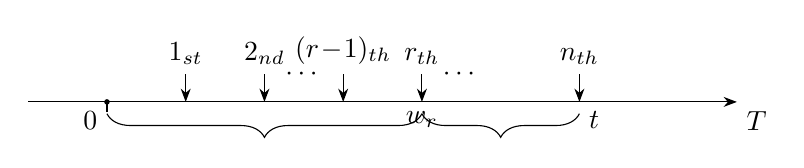
\begin{tikzpicture}[>=Stealth]
			\draw[->](-1,0)--(8,0)node[below right]{$T$};
			\fill (0,0)circle(1pt);
			\draw (0,-0.13)--(0,0)node[below left]{$0$};
			\draw[->] (1,0.35)node[above]{$1_{st}$}--(1,0);
			\draw[->] (2,0.35)node[above]{$2_{nd}$}--(2,0);
			\draw (2.5,0.35)node[]{$\cdots$};
			\draw[->](3,0.35)node[above]{$(r\!-\!1)_{th}$}--(3,0);
			\draw[->](4,0.35)node[above]{$r_{th}$}--(4,0)node[below]{$w_r$};
			\draw (4.5,0.35)node[]{$\cdots$};
			\draw[->](6,0.35)node[above]{$n_{th}$}--(6,0)node[below right]{$t$};
			\draw[decorate,decoration={brace,amplitude=3mm}] (4,-0.15)--(0,-0.15);
			\draw[decorate,decoration={brace,amplitude=3mm}] (6,-0.15)--(4,-0.15);
		\end{tikzpicture}
	\end{figure}
	将之分为三段,然后得到类似多项分布的结论(分三组乘起来)
	\[f_{W_r|N(t)=n}(w_r|n) = \frac{n!}{(r-1)!\cdot 1 \cdot (n-r)!}\left(\frac{w_r}{t}\right)^{r-1}\cdot \frac{1}{t}\cdot \left(\frac{t-w_r}{t}\right)^{n-r}\]
\end{solution}

\begin{problem}{2.8}
	令$\{N_i(t), t\geqslant 0\}, i = 1,2,\cdots, n$为n个独立的有相同强度参数$\lambda$的Possion过程. 记$T$为在全部$n$个过程中至少发生了一件事的时刻, 试求$T$的分布.
\end{problem}
\begin{solution}
	本题与1.14几乎一样,是Poisson和 \Exp 的一体两面.\\
	记$N(t)=N_1(t)+\cdots +N_n(t)\Rightarrow N(t)\sim \poi (n\lambda)$,其对应首达时$X\sim \Exp(n\lambda)$
	\begin{align*}
		F_T(t) & = \p[T \leqslant t] = 1 - \p(T<t)\\
			& = 1 - \p[N_i(t) = 0, i= 1, 2, \cdots, n]\\
			& = 1 - \left(\e^{-\lambda t}\right)^n
		\end{align*}
		$\therefore f_T(t) = F'_T(t) = n\lambda \e^{-n\lambda t}$\\
		即$T$服从参数为$n\lambda$的指数分布.
\end{solution}

\begin{problem}{2.9}
	考虑参数为$\lambda$的Possion过程$N(t)$, 若每一事件独立地以概率$p$被观察到, 并将观察到的过程记为$N_1(t)$. 试问$N_1(t)$是什么过程? $N(t)-N_1(t)$呢? $N_1(t)$与$N(t) - N_1(t)$是否独立?
\end{problem}
\begin{solution}
	由题设得
	\begin{enumerate}[label=(\roman*)]
		\item $N_1(0)=0$
		\item $\{N_1(t):t\geqslant 0\}$是独立增量过程
	\end{enumerate}
	从而对$0\leqslant s<t$,$N_1(t)-N_1(s)$服从参数为$\lambda p(t-s)$的Poisson分布.
	故$\{N_1(t):t\geqslant 0\}$是参数为$\lambda p$的Possion过程.
\end{solution}

\begin{problem}{2.10}
	到达某加油站的公路上的卡车服从参数为${\lambda}_1$的Possion过程$N_1(t)$, 而到达的小汽车服从参数为${\lambda}_2$的Possion过程$N_2(t)$, 且过程$N_1(t)$与$N_2(t)$独立. 试问随机过程$N(t) = N_1(t) + N_2(t)$是什么过程? 并计算在总车流数$N(t)$中卡车首先到达的概率.
\end{problem}
\begin{solution}
	\[g_N(v)  = g_{N_1}(v) \cdot g_{N_2}(v) = \e^{\lambda_1 v(\e^t-1)}\e^{\lambda_2 v(\e^t-1)} = \e^{(\lambda_1 +\lambda_2)\v(\e^t-1)}\]
	$\therefore N(t)$是强度为$\lambda_1+\lambda_2$的Possion过程\\
	记$W_1,W_2$分别为卡车、小汽车的第一次到达时间, 则$W_1$服从参数为$\lambda_1$的指数分布, $W_1$服从参数为$\lambda_1$的指数分布.
	\[\begin{split}
	\therefore P(W_1 < W_2) & = \iint\limits_{0 \leqslant W_1 < W_2 \leqslant +\infty}f_{W_1,W_2}(w_1,w_2)\d w_1\d w_2\\
	& = \int^{+\infty}_0\d w_1\int^{+\infty}_{w_1}\lambda_1\lambda_2\e^{-w_1\lambda_1-w_2\lambda_2}\,\d w_2\\
	& = \frac{\lambda_1}{\lambda_1+\lambda_2}
	\end{split}\]
\end{solution}

\begin{problem}{2.11}
	冲击模型(Shock Model)记$N(t)$为某系统到某时刻$t$受到的冲击次数, 它是参数为$\lambda$的Possion过程. 设第k次冲击对系统的损害大小$Y_k$服从参数为$\mu$的指数分布, $Y_k, k = 1, 2, \cdots, $独立同分布. 记$X(t)$为系统所受到的总损害. 当损害超过一定的极限$\alpha$时系统不能运行, 寿命终止, 记$T$为系统寿命. 试求该系统的平均寿命$\E(T)$, 并对所得结果作出直观解释.
	\par 提示:对非负随机变量$\displaystyle \E(T) = \int^\infty_0 \p(T>t)\d t$\\
\end{problem}
\begin{solution}[1]
	\[\begin{split}
	\p(T>t) & = \p\{X(t) \leqslant \alpha\} = \p\left\{\sum^{N(t)}_{k=1}Y_k \leqslant \alpha \right\}\\
	& = \sum^{\infty}_{n=0}\p\Bigg\{\sum^{N(t)}_{k=1}Y_k \leqslant \alpha \Bigg| N(t) = n\Bigg\} \cdot \p\{N(t) = n\}\\
	& = \sum^{\infty}_{n=0}\p\Bigg\{\sum^n_{k=1}Y_k \leqslant \alpha \Bigg| N(t) = n\Bigg\} \cdot \p\{N(t) = n\}\\
	& = \sum^{\infty}_{n=0}\p\{W_n \leqslant \alpha\} \cdot \p\{N(t) = n\}\\
	\end{split}\]
	求和式中当$n=0$时认为$\p\{W_n \leqslant \alpha | N(t) = n\} = 1$\\
	$\because Y_k \sim \Exp(\mu),\quad \therefore W_n = \sum\limits^n_{k=1}Y_k \sim \Gamma(n,\mu)$
	\[\begin{split}
	\p(W_n \leqslant \alpha) & = \frac{\mu^n}{(n-1)!}\int^\alpha_0s^{n-1}\e^{-\mu s}\d s\quad (n\geqslant 1)\\
	\p[N(t) = n] & = \frac{(\lambda t)^n}{n!}\e^{-\lambda t}
	\end{split}\]
	\[\therefore \p(T>t) = \e^{-\lambda t} + \e^{-\lambda t}\sum^{\infty}_{n=1}\frac{(\lambda\mu t)^n}{n!(n-1)!}\int^\alpha_0 s^{n-1}\e^{-\mu s}\d s\]
	\[\begin{split}
	\therefore \E(T) & = \int^{+\infty}_0 \p(T>t)\d t\\
	& = \frac{1}{\lambda} + \sum^{\infty}_{n=1}\frac{(\lambda\mu)^n}{n!(n-1)!}\int^{\infty}_0 t^n \e^{-\lambda t}\d t\int^\alpha_0 s^{n-1}\e^{-\mu s}\d s\\
	& = \frac{1}{\lambda} + \frac{1}{\lambda}\sum^{\infty}_{n=1}\frac{\mu^n\Gamma(n+1)}{n!(n-1)!}\int^\alpha_0 s^{n-1}\e^{-\mu s}\d s\\
	& = \frac{1}{\lambda} + \frac{1}{\lambda}\int^\alpha_0 \bigg[\sum^{\infty}_{n=1}\frac{(\mu s)^{n-1}\e^{-\mu s}}{(n-1)!}\bigg]\d (\mu s)\\
	& = \frac{1+\mu\alpha}{\lambda}
	\end{split}\]
	从结果看, 若$\lambda$越大(系统所受冲击越频繁), $\mu$越小(每次冲击所造成的平均损害越大), $\alpha$越小(系统所能承受的的损害极限越小), 则系统平均寿命越短, 且当$\alpha$等于$0$时系统的平均寿命即为第一次冲击到来的平均时间, 符合常识.
\end{solution}
\begin{solution}[2]
	\[G_n(\alpha) = \p\{Y_1+\cdots+Y_k \leqslant \alpha\} = \p\{W_n \leqslant \alpha\}= \p\{N_1(\alpha) \geqslant n\} = \sum^{\infty}_{k=n}\frac{(\mu\alpha)^n}{k!}\e^{-\mu\alpha}\]
	其中$N_1(t)$是强度为$\mu$的Possion过程\\
	\[\begin{split}
	\therefore \p(T>t) & = \p\{X(t) \leqslant \alpha\}\\
	& = \sum^{\infty}_{n=0}\frac{(\lambda t)^n \e^{-\lambda t}}{n!}G_n(\alpha) \qquad (\text{课本$\mathbf{P}_{21}$例2.4})\\
	& = \sum^{\infty}_{n=0}\sum^{\infty}_{k=n}\frac{(\lambda t)^n}{n!}\e^{-\lambda t}\frac{(\mu\alpha)^n}{k!}\e^{-\mu\alpha}\\
	& = \sum^{\infty}_{k=0}\frac{(\mu\alpha)^n}{k!}\e^{-\mu\alpha}\sum^{k}_{n=0}\frac{(\lambda t)^n}{n!}\e^{-\lambda t}
	\end{split}\]
	\[\begin{split}
	\therefore \E(T) & = \int^{+\infty}_0 \p(T>t)\d t\\
	& = \sum^{\infty}_{k=0}\frac{(\mu\alpha)^k}{k!}\e^{-\mu\alpha}\sum^{k}_{n=0}\int^{+\infty}_0\frac{(\lambda t)^n}{n!}\e^{-\lambda t}\d t\\
	& = \sum^{\infty}_{k=0}\frac{(\mu\alpha)^k}{k!}\e^{-\mu\alpha}\frac{(k+1)\Gamma(n+1)}{n!\lambda}\\
	& = \frac{1}{\lambda}\sum^{+\infty}_{k=0}\frac{(\mu\alpha)^k}{k!}\e^{-\mu\alpha} + \frac{\mu\alpha}{\lambda}\sum^{+\infty}_{k=1}\frac{(\mu\alpha)^{k-1}}{(k-1)!}\e^{-\mu\alpha}\\
	& = \frac{1+\mu\alpha}{\lambda}
	\end{split}\]
\end{solution}
\begin{solution}[3\footnote{Sol \textcolor{red}{3} 和Sol \textcolor{red}{4} 都是我写的,计算结果为$\frac{\mu \alpha}{\lambda}$.但实际结果应为$\frac{1+\mu \alpha}{\lambda}$,懒得去找漏项了}]
	\[\begin{aligned}
		1-F_T(t)&=\p(T<t)=\p[X(t)<\alpha ]=\p\left(\sum_{k=1}^{N(t)}Y_k\leq \alpha \right)\\
		& = \sum_{n=1}^{\infty}\p \left(\sum_{k=1}^{N(t)}Y_k\leq \alpha \Bigg|N(t)=n\right)\p [N(t)=n]\\
		& = \sum_{n=1}^{\infty}\p \left(\sum_{k=1}^{n}Y_k\leq \alpha \right)\p [N(t)=n]
	\end{aligned}\]
	$Y_1,Y_2,\dots ,Y_n\iid$且$Y_i\sim \Exp(\mu )$.设$S_n=\sum_{k=1}^{n}Y_k$
	由独立同分布的指数分布随机和为参数为$(n,\mu)$的$\Gamma$分布
	\[f_{S_n}(s)=\mu \frac{\e ^{-\mu s}(\mu s)^{n-1}}{(n-1)!}\]
	\[\p(S_n\leq \alpha)=\int_{0}^{\alpha}\mu \frac{\e ^{-\mu s}(\mu s)^{n-1}}{(n-1)!}\d s=\frac{\mu}{(n-1)!}\int_{0}^{\alpha}\e^{-\mu s}(\mu s)^{n-1}\d s\]
	\[\begin{aligned}
		1-F_T(t)&=\sum_{n=1}^{\infty}\frac{\e ^{-\lambda t}(\lambda t)^n}{n!}\cdot \frac{\mu}{(n-1)!}\int_{0}^{\alpha}\e^{-\mu s}(\mu s)^{n-1}\d s\\
		&=\mu \e^{-\lambda t}\sum_{n=1}^{\infty}\int_{0}^{\alpha}\frac{(\lambda t)^n}{n!(n-1)!}\e^{-\mu s}(\mu s)^{n-1}\d s\\
		&\xlongequal{\text{\textcolor{red}{交换求和和积分符号}}}\mu \e^{-\lambda t}\int_{0}^{\alpha}\sum_{n=0}^{\infty}\frac{(\lambda t)^{n+1}}{(n+1)!}\frac{(\mu s)^n\e^{-\mu s}}{n!}\d s\\
	\end{aligned}\]
	因为$\displaystyle \sum_{n=0}^{\infty}\frac{(\lambda t)^{n+1}}{(n+1)!}=\e^{\lambda t}-1 ,\quad \sum_{n=0}^{\infty}\frac{(\mu s)^n \e^{-\mu s}}{n!}=1$
	\\ 所以由\textcolor{red}{Mertens定理}得$\displaystyle \sum_{n=0}^{\infty}\frac{(\lambda t)^{n+1}}{(n+1)!}\frac{(\mu s)^n \e^{-\mu s}}{n!}=(\e^{\lambda t}-1)\cdot 1=\e^{\lambda t}-1$
	\[\begin{aligned}
		1-F_T(t)&=\mu \e^{-\lambda t}\int_{0}^{\alpha}(\e^{\lambda t}-1)\cdot 1\d s=\mu \alpha (1-\e^{-\lambda t})\\
		f_T(t)&=-\frac{\d}{\d t}(1-F_T(t))=\lambda \mu \alpha \e^{-\lambda t}\\
		\E(T)&=\int_{0}^{+\infty}t f_T(t)\d t=\frac{\mu \alpha}{\lambda }
	\end{aligned}\]
\end{solution}
\begin{solution}[4\footnote{请查看上页的脚注}]
	可以采用不那么暴力的方法,即使用题目里的提示$\displaystyle \E(T)=\int_{0}^{+\infty}\p(T>t)\d t$,
    先把这个提示证一遍
    \[\begin{aligned}
    	\int_{0}^{+\infty}\p(T>t)\d t &=\int_{0}^{+\infty}\left(\int_{t}^{+\infty}f_T(x)\d x\right)\d t\xlongequal{\text{交换积分次序}}\\
        &=\int_{0}^{+\infty}\d x \int_{0}^{x}f_T(x)\d t=\int_{0}^{+\infty}xf_T(x)\d x=\int_{0}^{+\infty}tf_T(t)\d t\\
        &=\E(T)
    \end{aligned}\]
    \[\begin{aligned}
        \p(T>t)&=1-F_T(t)=\mu \e^{-\lambda t}\int_{0}^{\alpha}\sum_{n=0}^{\infty}\frac{(\lambda t)^{n+1}}{(n+1)!}\frac{(\mu s)^n \e^{-\mu s}}{n!}\d s\\
        \E(T)&=\int_{0}^{+\infty}\p(T>t)\d t\\
        &=\sum_{n=1}^{\infty}\frac{(\mu \lambda)^n}{n!(n-1)!}\int_{0}^{+\infty}t^n \e^{-\lambda t}\d t\cdot \int_{0}^{\alpha}s^{n-1}\e^{-\mu s}\d s\\
        &=\frac{1}{\lambda}\sum_{n=1}^{\infty}\frac{\mu ^n}{(n-1)!}\int_{0}^{\alpha}s^{n-1}\e^{-\mu s}\d s\\
        &=\frac{1}{\lambda}\int_{0}^{\alpha}\e^{-\mu s}\sum_{n=1}^{\infty}\frac{\mu ^n}{(n-1)!}s^{n-1}\d s\\
        &=\frac{\mu}{\lambda}\int_{0}^{\alpha}\d s=\frac{\mu \alpha}{\lambda}
    \end{aligned}\]
\end{solution}

\begin{problem}{2.12}
	令$N(t)$是强度函数为$\lambda (t)$的非齐次Possion过程, $X_1, X_2, \cdots$为事件间的时间间隔.
	\begin{enumerate}[label=(\roman*)]
		\item $X_i$是否独立;
		\item $X_i$是否同分布;
		\item 试求$X_1$与$X_2$的分布.
	\end{enumerate}
\end{problem}
\begin{solution}[1]
	记$\displaystyle m(t) = \int^t_0\lambda(u)\d u$
	等待时间$W_1,W_2$的联合分布函数为
	\[\begin{split}
		F_{W_1,W_2}(t_1,t_2) & = \p(W_1 \leqslant t_1, W_2 \leqslant t_2),\qquad (0\leqslant t_1 < t_2)\\
		& = \p(N(t_1) \geqslant 1, N(t_2) \geqslant 2)\\
		& = \sum^{\infty}_{k=2}\sum^k_{\ell=1}\p[N(t_1) = \ell, N(t_2) = k]\\
		& = \sum^{\infty}_{k=2}\sum^k_{\ell=1}\p[N(t_1) = \ell, N(t_2) - N(t_1) = k - \ell]\\
		& = \sum^{\infty}_{k=2}\sum^k_{\ell=1}\p[N(t_1) = \ell)\p(N(t_2) - N(t_1) = k - \ell]\\
		& = \sum^{\infty}_{k=2}\sum^k_{\ell=1}\frac{(m(t_1)^\ell)}{\ell !}\e^{-m(t_1)}\cdot \frac{[m(t_2)-m(t_1)]^{k-\ell}}{(k-\ell)!}\e^{-[m(t_2)-m(t_1)]}\\
		& = \sum^{\infty}_{k=2}\sum^k_{\ell=1}\frac{(m(t_1))^\ell[m(t_2)-m(t_1)]^{k-\ell}}{\ell !(k-\ell)!}\e^{-m(t_2)}\\
		& = \e^{-m(t_2)}\sum^{\infty}_{k=2}\frac{1}{k!}\sum^k_{\ell=1}\binom{k}{\ell}[m(t_1)]^\ell[m(t_2)-m(t_1)]^{k-\ell}\\
		& = \e^{-m(t_2)}\sum^{\infty}_{k=2}\frac{1}{k!}\bigg\{\sum^k_{\ell=0}\binom{k}{\ell}[m(t_1)]^\ell[m(t_2)-m(t_1)]^{k-\ell}-[m(t_2)-m(t_1)]^k\bigg\}\\
		& = \e^{-m(t_2)}\Big\{\e^{m(t_2)}-\e^{m(t_2)-m(t_1)}-m(t_1)\Big\}\\
		& = 1-\e^{-m(t_1)}-m(t_1)\e^{-m(t_2)}\\
	\end{split}\]
	\[\therefore f_{W_1,W_2}(t_1,t_2) = \frac{\partial^2F_{W_1,W_2}(t_1,t_2)}{\partial t_1\partial t_2} = \lambda(t_1)\lambda(t_2)\e^{-m(t_2)}\]
	\[\because
	\begin{cases}
	W_1 = X_1\\
	W_2 = X_1 + X_2
	\end{cases}\]
	$\therefore f_{X_2,X_2}(t_1,t_2) = \lambda(t_1)\lambda(t_1+t_2)\e^{-m(t_1+t_2)}$不能写为$g_1(t_1)g_2(t_2)$形式\\
	$\therefore X_1, X_2$不独立,又有
	\[f_{X_1}(t_1) = \lambda(t_1)\int^{+\infty}_0\lambda(t_1+t_2)\e^{-m(t_1+t_2)}\d t_2 = \lambda(t_1)\Big[\e^{-m(t_1)}-\e^{-m(+\infty)}\Big]\quad (t_1 > 0)\]
	下面确定$\e^{-m(\infty)}$:
	\[1 = \int^{+\infty}_0f_{X_1}(t_1)\d t_1 = \int^{+\infty}_0\lambda(t_1)\Big[\e^{-m(t_1)}-\e^{-m(+\infty)}\Big]\d t_1 = 1 - [m(+\infty)+1]\e^{-m(+\infty)}\]
	$\therefore \e^{-m(+\infty)} = 0$
	\[\begin{split}
	\therefore f_{X_1}(t_1) & = \lambda(t_1)\e^{-m(t_1)}\qquad (t_1>0)\\
	f_{X_2}(t_2) & = \int^{+\infty}_0\lambda(t_1)\lambda(t_1+t_2)\e^{-m(t_1+t_2)}\d t_1 \qquad (t_2>0)\\
	\end{split}\]
	$\therefore X_1,X_2$不同分布且其概率密度函数如上.
\end{solution}

\begin{problem}{2.13}
	考虑对所有$t$, 强度函数$\lambda (t)$均大于$0$的非齐次Possion过程$\{N(t), t \geqslant 0\}$. 令$\displaystyle m(t) = \int^t_0 \lambda(u)\d u, m(t)$的反函数为$\ell(t)$, 记$N_1(t)= N(\ell(t))$. 试证$N_1(t)$是通常的Possion过程, 试求$N_1(t)$的强度参数$\lambda$.
\end{problem}
\begin{solution}
	\begin{enumerate}[label=(\roman*)]
		\item $N_1(0)=N(\ell(0))=N(0)=0$
		\item $\because m(\ell)$单增, $\therefore \ell(t)$单增\\
			$\therefore $对任意$0 \leqslant t_1 < t_2 \cdots < t_n$, 有$0 \leqslant \ell(t_1) < \ell(t_2) < \cdots < \ell(t_n)$,且有
			\begin{align*}
				N_1(t_2) - N_1(t_1) & = N(\ell(t_2)) - N(\ell(t_1))\\
				N_1(t_3) - N_1(t_2) & = N(\ell(t_3)) - N(\ell(t_2))\\
				\vdots \\
				N_1(t_n) - N_1(t_{n-1}) & = N(\ell(t_n)) - N(\ell(t_{n-1}))
			\end{align*}
			$\because N(t)$是独立增量过程 \quad $\therefore N_1(t)$也是独立增量过程
		\item $\forall \,0 \leqslant s < t$, 有
			\[\begin{split}
				\p(N_1(t) - N_1(s) = k) & = \p\{N(\ell(t)) - N(\ell(s)) = k\}\\
				& = \frac{[m(\ell(t)) - m(\ell(s))]^k}{k!} \e^{-[m(\ell(t)) - m(\ell(s))]}\\
				& = \frac{(t-s)^k}{k!}\e^{-(t-s)} \qquad (k=0,1,\cdots)
			\end{split}\]
			$\therefore N_1(t)$是强度为$1$的Possion过程
	\end{enumerate}
\end{solution}

\begin{problem}{2.14}
	设$N(t)$为更新过程, 试判断下述命题的真伪:
	\begin{enumerate}[label=(\roman*)]
		\item $\{N(t) < k \} \Longleftrightarrow \{W_k > t\}$;
		\item $\{N(t) \leqslant k \} \Longleftrightarrow \{W_k \geqslant t\}$;
		\item $\{N(t) > k \} \Longleftrightarrow \{W_k < t\}$;
	\end{enumerate}
	其中$W_k$为第$k$个事件的等待时间.
\end{problem}
\begin{solution}
	\begin{enumerate}[label=(\roman*)]
		\item $\displaystyle \{N(t) < k \} = \overline{\{N(t) \geqslant k\}} = \overline{\{W_k \leqslant t\}} = \{W_k > t\}$
		\item \[\begin{split}
				\{N(t) \leqslant k \} & = \{N(t) < k + 1\} = \overline{\{N(t) \geqslant k + 1\}} = \overline{\{W_{k+1} \leqslant t\}}\\
				& = \{W_{k+1} > t\} \neq \{W_k \geqslant t\}
			  \end{split}\]
			  \begin{figure}[H]
				\centering
				\begin{tikzpicture}[>=Stealth]
					\draw[->](-0.5,0)--(0,0)node[below]{0}--(6,0)node[below right]{$T$};
					\fill (0,0)circle(1pt);
					\draw[->] (1,0.35)node[above]{$1_{st}$}--(1,0);
					\draw[->] (2,0.35)node[above]{$2_{nd}$}--(2,0);
					\draw (2.5,0.35)node[]{$\cdots$};
					\draw[->](3,0.35)node[above]{$k_{th}$}--(3,0);
					\draw[->](5,0.35)node[above]{$(k\!+\!1)_{th}$}--(5,0);
					\fill (3,0)node[below]{$W_k$}circle(1pt);
					\fill (4,0)node[below]{$t$}circle(1pt);
					\draw (6.5,0)node[above right]{$N(t)=k$但$W_k<t$};
					\draw (6.5,0)node[below right]{$W_k<t$但$N(t)=k$};
			  	\end{tikzpicture}
		  	  \end{figure}
			  故$\{N(t)\leqslant k\}\nRightarrow \{W_k\leq t\}$
		\item $\displaystyle \{N(t) > k \} = \{N(t) \geqslant k+1\} = \{W_{k+1} \leqslant t\} \neq \{W_k < t\}$
			  \\ 同样参照上图,$\{W_k<t\}\nRightarrow \{N(t)>k\}$
	\end{enumerate}
\end{solution}

\clearpage
\section{第三章 Markov过程}
\begin{problem}{3.1}
	对Markov链$X_n,n\geqslant 0$,试证条件\[\p(X_{n+1}=j|X_0=i_0,\dots ,X_{n-1}=i_{n-1},X_n=i)=\p(X_{n+1}=j|X_n=i)\]
	等价于对所有时刻$n,m$及所有状态$i_0,\dots , i_n,j_1,\dots ,j_m$有
	\[\begin{aligned}
		& \p(X_{n+1}=j_1,\dots ,X_{n+m}=j_m|X_0=i_0, \dots , X_n=i_n)\\
		= &\p(X_{n+1}=j_1,\dots ,X_{n+m}=j_m|X_n=i_n)
	\end{aligned}\]
\end{problem}
\begin{solution}
	$\Leftarrow $只需令$m=1$\\
	$\Rightarrow $由$\mathbf{P}_{27}(3.4)$可知
	\[\begin{split}
	& \quad P\{X_{n+1} = j_1, \cdots, X_{n+m} = j_m | X_0 = i_0, \cdots, X_n = i_n\}\\
	& = P\{X_{n+1} = j_1, \cdots, X_{n+m} = j_m , X_0 = i_0, \cdots, X_n = i_n\} / P\{X_0 = i_0, \cdots, X_n = i_n\}\\
	& = P\{X_0 = i_0\} \cdot P_{j_1j_2} \cdots P_{j_{m-1}j_m} P_{i_0i_1} \cdots P_{i_1j_1} / [P\{X_0 = i_0\} \cdot P_{i_0i_1} \cdots P_{i_{n-1}i_n}\\
	& = P\{X_n = i\} \cdot P_{j_1j_2} \cdots P_{j_{m-1}j_m} P_{i_nj_1} / P\{X_n = i_n\}\\
	& = P\{X_{n+1} = j_1, \cdots, X_{n+m} = j_m | X_n = i_n\}\\
	\end{split}\]
\end{solution}

\begin{problem}{3.2}
	考虑状态 $ 0,1,2 $ 上的一个Markov链$X_n, n \geqslant 0$, 它有转移概率矩阵
	\[\bm{P} = \begin{pmatrix}
	0.1 & 0.2 & 0.7 \\
	0.9 & 0.1 & 0 \\
	0.1 & 0.8 & 0.1
	\end{pmatrix}\]
	初始分布为$p_0 = 0.3, p_1 = 0.4, p_2 = 0.3$, 试求概率$P\{X_0 = 0, X_1 = 1, X_2 = 2\}$.
\end{problem}
\begin{solution}
	\[\p\{X_0 = 0, X_1 = 1, X_2 = 2\} = p_0P_{01}P_{12} = 0.3 \times 0.1 \times 0 = 0\]
\end{solution}

\begin{problem}{3.3}
	信号传送问题. 信号只有 $0,1$ 两种, 分为多个阶段传输. 在每一步上出错的概率为$\alpha$. $X_0 = 0$是送出的信号, 而$X_n$是在第$n$步接收到的信号. 假定$X_n$为一Markov链,它有转移概率矩阵$P_{00} = P_{11} = 1-\alpha,\,P_{01} = P_{10} = \alpha,\, 0<\alpha <1$.试求
	\begin{enumerate}[label=(\alph*)]
		\item 两步均不出错的概率$\p\{X_0 = 0, X_1 = 0, X_2 = 0\}$;
		\item 两步传送后收到正确信号的概率;
		\item 五步之后传送无误的概率$\p\{X_5 = 0 | X_0 = 0\}$.
	\end{enumerate}
\end{problem}
\begin{solution}
	\begin{enumerate}[label=(\alph*)]
		\item $\p\{X_0 = 0, X_1 = 0, X_2 = 0\} = p_0P_{00}P_{00} = 1 \cdot (1-\alpha) \cdot (1-\alpha) = (1-\alpha)^2$
		\item $P = p_0P_{00}P_{00} + p_0P_{01}P_{10} = (1-\alpha)^2 + {\alpha}^2 = 2{\alpha}^2 - 2\alpha + 1$
		\item 转移概率矩阵
			\[\bm{P} = \begin{pmatrix} \frac{\sqrt{2}}{2} & \frac{\sqrt{2}}{2}\\ \frac{\sqrt{2}}{2} & -\frac{\sqrt{2}}{2} \end{pmatrix}^{-1}
			\begin{pmatrix} 1 & 0 \\ 0 & 1-2\alpha \end{pmatrix}
			\begin{pmatrix} \frac{\sqrt{2}}{2} & \frac{\sqrt{2}}{2}\\ \frac{\sqrt{2}}{2} & -\frac{\sqrt{2}}{2} \end{pmatrix}\]
			\[\begin{aligned}
			\therefore \bm{P}^{(5)} & =
				\begin{pmatrix} \frac{\sqrt{2}}{2} & \frac{\sqrt{2}}{2}\\ \frac{\sqrt{2}}{2} & -\frac{\sqrt{2}}{2} \end{pmatrix}^{-1}
				\begin{pmatrix} 1 & 0 \\ 0 & (1-2\alpha)^5 \end{pmatrix}
				\begin{pmatrix} \frac{\sqrt{2}}{2} & \frac{\sqrt{2}}{2}\\ \frac{\sqrt{2}}{2} & -\frac{\sqrt{2}}{2} \end{pmatrix}\\
							& = \begin{pmatrix}
							\frac{1+(1-2\alpha)^5}{2} & \frac{1-(1-2\alpha)^5}{2}\\ \frac{1-(1-2\alpha)^5}{2}& \frac{1+(1-2\alpha)^5}{2}
							\end{pmatrix}
			\end{aligned}\]
			$\therefore \p\{ X_5 = 0 | X_0 = 0\} = p_0 \cdot \frac{1+(1-2\alpha)^5}{2} = \frac{1+(1-2\alpha)^5}{2}$\\
			或者直接\[\p\{X_5=0|X_0=0\}=(1-\alpha)^5 +\binom{5}{2}(1-\alpha)^3 \alpha ^2 +\binom{5}{4}(1-\alpha )\alpha ^4\]
	\end{enumerate}
\end{solution}

\begin{problem}{3.4}
	$A, B$ 两罐总共装各 $N$ 个球. 作如下实验:在时刻 $n$ 先 $n$ 个球中等概率地任取一球. 然后从 $A, B$ 两罐中任选一个, 选中 $A$ 的概率为 $p$, 选中 $B$ 的概率为 $q$. 之后再将选出的球放入选好的罐中. 设 $X_n$ 为每次试验时 $A$ 罐中的球数. 试求此Markov过程的转移概率矩阵.
\end{problem}
\begin{solution}
	\[P_{ij} =
	\begin{cases}
	p \cdot \frac{i}{N} + q \cdot \frac{N-i}{N} & , j = i\\
	q \cdot \frac{i}{N} & , j = i-1(i=1,2,\cdots ,N)\\
	p \cdot \frac{N-i}{N} & , j = i+1(i=0,1,\cdots ,N-1)\\
	0 & , \text{其他}
	\end{cases}\]
	其转移概率矩阵为
	\[\bm{P} = \frac{1}{N}
	\begin{pmatrix}
	qN & pN & 0 & \cdots & 0 & 0 & 0 \\
	q & q(N-1)+p & p(N-1) & \cdots & 0 & 0 & 0 \\
	0 & 2q & q(N-2)+2p & \cdots & 0 & 0 & 0\\
	\vdots & \vdots & \vdots & \ddots & \vdots & \vdots & \vdots \\
	0 & 0 & 0 & \cdots & 2q+p(N-2) & 2p & 0\\
	0 & 0 & 0 & \cdots & q(N-1) & q+p(N-1) & p\\
	0 & 0 & 0 & \cdots & 0 & qN & pN
	\end{pmatrix}\]
\end{solution}

\begin{problem}{3.5}
	重复掷币一直到连续出现两次正面为止. 假定钱币是均匀的, 试引入以连续出现次数为状态空间的Markov链, 并求出平均需要掷多少次试验才可以结束.
\end{problem}
\begin{solution}[1]
	记$X_n$为第$n$次掷币后连续出现的正面次数, 则$\{X_n, n \geqslant 0 \}$为一M.C.\\
	其转移概率矩阵为
	$\bm{P} = \bordermatrix{
		~ & 0 & 1 & 2 \cr
		0 & \frac{1}{2} & \frac{1}{2} & 0 \cr
		1 & \frac{1}{2} & 0 & \frac{1}{2} \cr
		2 & 0 & 0 & 1}$
	\[\begin{split}
	\therefore & \quad \E(T | X_0 = 0)\\
			& = \sum^2_{k=0}\E(T|X_0 = 0, X_1 = k)\cdot \p(X_1 = k | X_0 = 0)\\
			& = \sum^2_{k=0}\E(T|X_1 = k)\cdot \p(X_1 = k | X_0 = 0)\\
			& = (1+v)\cdot \frac{1}{2} + \E(T| X_1 = 1) \cdot \frac{1}{2}\\
	\text{及}& \quad \E(T | X_1 = 1)\\
			& = \sum^2_{k=0}\E(T|X_1 = 1, X_2 = k)\cdot \p(X_2 = k | X_1 = 1)\\
			& = \sum^2_{k=0}\E(T|X_2 = k)\cdot \p(X_2 = k | X_1 = 1)\\
			& = (2+v)\cdot \frac{1}{2} + 0 + \frac{1}{2} \times 2
	\end{split}\]
	解得$\E(T | X_0 = 0) = 6$, 平均需掷$6$次.
\end{solution}
\begin{solution}[2]
	由转移概率矩阵,有$P_{00}=\frac{1}{2}, P_{01}=\frac{1}{2},P_{10}=\frac{1}{2},P_{12}=\frac{1}{2}$,则
	\[\begin{aligned}
		\E(N) & = \sum_{n=0}^{\infty}\sum_{k=0}^{n}\binom{n}{k}P_{00}^k (P_{01}P_{10})^{n-k}[k+2(n-k)+2]\cdot P_{01}P_{12}\\
		& = \frac{1}{4}\sum_{n=0}^{\infty}\sum_{k=0}^{n}\binom{n}{k}\left(\frac{1}{2}\right)^k \left(\frac{1}{4}\right)^{n-k}[k+2(n-k)+2]\\
		& = \frac{1}{4}\times 24 = 6
	\end{aligned}\]
\end{solution}

\begin{problem}{3.6}
	迷宫问题. 将小家鼠放入迷宫内作动物的学习试验, 如下图所示. 在迷宫的第$7$号小格内放有美味食物而第$8$号小格内则是电击捕鼠装置. 假定当家鼠位于某格时有$k$个出口可以离去, 则它总是随机地选择一个, 概率为$1/k$. 并假定每一次家鼠只能跑到相邻的小格去. 令过程$X_n$为家鼠在时刻$n$时所在小格的号码, 试写出这一Markov过程的转移概率阵, 并求出家鼠在遭到电击前能找到食物的概率.
	\begin{figure}[H]
		\centering
		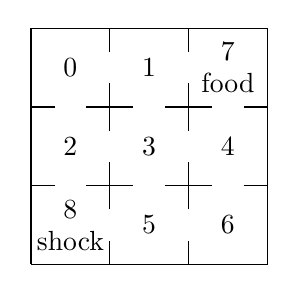
\begin{tikzpicture}
			\draw (0,0)--(3,0)--(3,3)--(0,3)--(0,0);
			\draw (1,0)--(1,0.3) (1,0.7)--(1,1.3) (1,1.7)--(1,2.3) (1,2.7)--(1,3);
			\draw (2,0)--(2,0.3) (2,0.7)--(2,1.3) (2,1.7)--(2,2.3) (2,2.7)--(2,3);
			\draw (0,1)--(0.3,1) (0.7,1)--(1.3,1) (1.7,1)--(2.3,1) (2.7,1)--(3,1);
			\draw (0,2)--(0.3,2) (0.7,2)--(1.3,2) (1.7,2)--(2.3,2) (2.7,2)--(3,2);
			\draw (0.5,2.5)node[]{0} (1.5,2.5)node[]{1} (2.5,2.7)node[]{7} (2.5,2.3)node[]{food};
			\draw (0.5,1.5)node[]{2} (1.5,1.5)node[]{3} (2.5,1.5)node[]{4};
			\draw (0.5,0.7)node[]{8} (0.5,0.3)node[]{shock} (1.5,0.5)node[]{5} (2.5,0.5)node[]{6};
		\end{tikzpicture}
	\end{figure}
\end{problem}
\begin{solution}
	\[
	\bm{P} =
	\bordermatrix{
		~ & 0 & 1 & 2 & 3 & 4 & 5 & 6 & 7 & 8 \cr
		0 & 0 & \frac{1}{2} & \frac{1}{2} & 0 & 0 & 0 & 0 & 0 & 0 \cr
		1 & \frac{1}{3} & 0 & 0 & \frac{1}{3} & 0 & 0 & 0 & \frac{1}{3} & 0 \cr
		2 & \frac{1}{3} & 0 & 0 & \frac{1}{3} & 0 & 0 & 0 & 0 & \frac{1}{3}\cr
		3 & 0 & \frac{1}{4} & \frac{1}{4} & 0 & \frac{1}{4} & \frac{1}{4} & 0 & 0 & 0 \cr
		4 & 0 & 0 & 0 & \frac{1}{3} & 0 & 0 &\frac{1}{3} & \frac{1}{3} & 0 \cr
		5 & 0 & 0 & 0 & \frac{1}{3} & 0 & 0 &\frac{1}{3} & 0 & \frac{1}{3} \cr
		6 & 0 & 0 & 0 & 0 & \frac{1}{2} & \frac{1}{2} & 0 & 0 & 0 \cr
		7 & 0 & 0 & 0 & 0 & 0 & 0 & 0 & 1 & 0 \cr
		8 & 0 & 0 & 0 & 0 & 0 & 0 & 0 & 0 & 1 \cr}
	\]
	设$u_k$为家鼠从$k$出发在遭到电击前能找到食物的概率, 显然$u_7 = 1, u_8 = 0$\\
	设$T$为进入吸收态时刻, 则当$0 \leqslant k \leqslant 6$时,
	\begin{align*}
	u_k & = \p\{X_T = 7 | X_0 = k\}\\
		& = \sum^8_{i=0}\p\{X_T = 7, X_1 = i | X_0 = k\}\\
		& = \sum^8_{i=0}\p\{X_T = 7, X_1 = i\} \p\{X_1 = i | X_0 = k\}
	\end{align*}
	\[\therefore
		\begin{cases}
		u_0 = \frac{1}{2}(u_1+u_2)\\
		u_1 = \frac{1}{3}(u_0+u_3+u_7)\\
		u_2 = \frac{1}{3}(u_0+u_3+u_8)\\
		u_3 = \frac{1}{4}(u_1+u_2+u_4+u_5)\\
		u_4 = \frac{1}{3}(u_3+u_6+u_7)\\
		u_5 = \frac{1}{3}(u_3+u_6+u_8)\\
		u_6 = \frac{1}{2}(u_4+u_5)\\
		u_7 = 1\\
		u_8 = 0
		\end{cases}\Rightarrow
		\begin{cases}
		u_0 = \frac{1}{2}\\
		u_1 = \frac{2}{3}\\
		u_2 = \frac{1}{3}\\
		u_3 = \frac{1}{2}\\
		u_4 = \frac{2}{3}\\
		u_5 = \frac{1}{3}\\
		u_6 = \frac{1}{2}\\
		u_7 = 1\\
		u_8 = 0
		\end{cases}
	\]
\end{solution}

\begin{problem}{3.7}
	记$Z_i, i = 1, 2, \cdots$ 为一串独立同分布的离散随机变量. $\p\{Z_1 = k\} = p_k \geqslant 0, k = 0,1,2,\cdots, \sum\limits^\infty_{k=0} = 1$. 记$X_n = Z_n, n = 1, 2, \cdots$. 试求过程$X_n$的转移概率矩阵.
\end{problem}
\begin{solution}
	$\because \p\{X_{n+1} = i_{n+1} | X_1 = i_1, \cdots , X_n = i_n\} = \p\{X_{n+1} = i_{n+1}\}$\\
	$\p\{X_{n+1} = i_{n+1} | X_n = i_n\} = \p\{X_{n+1} = i_{n+1}\}$\\
	$\therefore \p\{X_{n+1} = i_{n+1} | X_1 = i_1, \cdots , X_n = i_n\} = \p\{X_{n+1} = i_{n+1} | X_n = i_n\}$\\
	$\therefore \{X_n\}$是一M.C.,其转移概率矩阵为
	\[\bm{P} =
		\begin{pmatrix}
			p_0 & p_1 & p_2 & \cdots \\
			p_0 & p_1 & p_2 & \cdots \\
			p_0 & p_1 & p_2 & \cdots \\
			\vdots & \vdots & \vdots & \ddots
	\end{pmatrix}\]
\end{solution}

\begin{problem}{3.8}
	对第7题中的$Z_i$, 令$X_n = \max \{Z_1, \cdots , Z_n\}, n = 1, 2, \cdots$, 并约定$X_0 = 0$. $X_n$是否为Markov链? 如果是, 其转移概率阵是什么?
\end{problem}
\begin{solution}
	\begin{align*}
		X_{n+1} & = \max \{Z_1, \cdots, Z_n, Z_{n+1}\}\\
		& = \max \{\max\{Z_1, \cdots, Z_n\}, Z_{n+1}\}\\
		& = \max \{X_n, Z_{n+1}\}
	\end{align*}
	$\therefore \{X_n\}$是M.C.
	\[
		P_{ij} =
		\begin{cases}
			0 & , j < i\\
			p_j & , j > i\\
			\sum\limits^i_{k=0}p_k & , j = i\\
			0 & , \text{其他}
		\end{cases}
	\]
	其转移概率矩阵为
	\[
		\bm{P} =
		\begin{pmatrix}
			p_0 & p_1 & p_2 & \cdots \\
			0 & p_0+p_1 & p_2 & \cdots \\
			0 & 0 & p_0+p_1+p_2 & \cdots \\
			\vdots & \vdots & \vdots & \ddots
		\end{pmatrix}
	\]
\end{solution}

\begin{problem}{3.9}
	设$f^{(n)}_{ij}$表示从$i$出发在$n$步转移时首次到达$j$的概率, 试证明
	\[P^{(n)}_{ij} = \sum^n_{k=0}f^{(k)}_{ij}P^{(n-k)}_{jj}.\]
\end{problem}
\begin{solution}[1]
	设$T_j = \min \{n: n \geqslant 0 \,\text{且}\, X_n = j\}$
	\[\begin{split}
		\therefore P^{(n)}_{ij} & = \p\{X_n = j | X_0 = i\} = \sum^n_{k=0}\p\{X_n = j, T_j = k | X_0 = i\}\\
		& = \sum^n_{k=0}\p\{T_j = k | X_0 = i\}P^{(n-k)}_{jj}\\
		& = \sum^n_{k=0}\p\{X_k = j, X_s\neq j(s = 0,1,\cdots, k-1) | X_0 = i\}P^{(n-k)}_{jj}\\
		& = \sum^n_{k=0}f^{(k)}_{ij} P^{(n-k)}_{jj}
	\end{split}\]
\end{solution}
\begin{solution}[2(郑老师解法)]
	\[\begin{aligned}
		& P_{ij}^{(n)}=\p\{X_n=j|X_0=i\}\\
		= & \p\{\underbrace{X_n=j}_{\color{red}C},\underbrace{X_1=j}_{\color{red}B}|\underbrace{X_0=i}_{\color{red}A}\} + \p\{X_n=j,X_1\neq j|X_0=i\}\xlongequal{\color{red}\p(BC|A)=\p(B|A)\p(C|AB)} \\
		= & \p\{X_n=j|X_0=i,X_1=j\}P_{ij} + \p\{X_n=j,X_1\neq j|X_0=i\}\\
		= & f_{ij}^{(1)}P_{jj}^{(n-1)} + \p\{X_n=j,X_1\neq j|X_0=i\}\\
		= & f_{ij}^{(1)}P_{jj}^{(n-1)} + \p\{\underbrace{X_n=i}_{\color{red}C},\underbrace{X_2=j,X_1\neq j}_{\color{red}B}|\underbrace{X_0=i}_{\color{red}A}\} + \p\{X_n=j,X_2\neq j,X_1\neq j|X_0=i\}\\
		= & f_{ij}^{(1)}P_{jj}^{(n-1)} + \p\{X_2=j,X_1\neq j|X_0=i\}\p\{X_n=j|X_0=i,X_1\neq j,X_2=j\}\\
		  & +\p\{X_n=j,X_2\neq j,X_1\neq j|X_0=i\}\\
		= & f_{ij}^{(1)}P_{jj}^{(n-1)} + f_{ij}^{(2)}P_{jj}^{(n-2)} + \p\{X_n=j,X_2\neq j,X_1\neq j|X_0=i\} = \cdots \\
		= & \sum_{k=1}^{n-1}f_{ij}^{(k)}P_{jj}^{(n-k)} + \p\{X_n=j,X_k\neq j,k=1,2,\dots , n-1|X_0=i\}\\
		= & \sum_{k=1}^{n-1}f_{ij}^{(k)}P_{jj}^{(n-k)} + f_{ij}^{(n)}P_{jj}^{(0)}\\
		= & \sum_{k=1}^{n}f_{ij}^{(k)}P_{jj}^{(n-k)}
	\end{aligned}\]
\end{solution}

\begin{problem}{3.10}
	对第7题中的$Z_i$, 若定义$X_n = \sum\limits^n_{i=1}Z_i, n = 1, 2, \cdots, X_0 = 0$, 试证$X_n$为Markov链. 并求其转移概率矩阵.
\end{problem}
\begin{solution}
	对$n \geqslant 0$有
	\[\begin{split}
		& \quad \p\{X_{n+1} = i_{n+1} | X_0 = i_0, \cdots, X_n = i_n\} \qquad (i_0 = 0)\\
		& = \p\{Z_{n+1} = i_{n+1} - i_n | X_0 = i_0, \cdots, X_n = i_n\}\\
		& = \p\{Z_{n+1} = i_{n+1} - i_n\}\\
		& = \begin{cases}
		P_{i_{n+1}-i_n} &, i_{n+1} - i_n = 0,1,2,\cdots\\
		0 &, ow
		\end{cases}
	\end{split}\]
	\[\begin{split}
			& \{X_{n+1} = i_{n+1} | X_n = i_n\}\\
		= & \p\{X_{n} + Z_{n+1} = i_{n+1} | X_n = i_n\}\\
		= & \p\{Z_{n+1} = i_{n+1} - i_n\}
	\end{split}\]
	$\therefore X_n $是M.C.
	\[\bm{P} =
		\begin{pmatrix}
			p_0 & p_1 & p_2 & \cdots \\
			0	& p_0 & p_1 & \cdots \\
			0	& 0	  & p_0 & \cdots \\
			\vdots & \vdots & \vdots & \ddots
		\end{pmatrix}
	\]
\end{solution}

\begin{problem}{3.11}
	一Markov链有状态$0,1,2,3$和转移概率矩阵
	\[
		\bm{P} =
		\begin{pmatrix}
			0 & \frac{1}{2} & 0 & \frac{1}{2}\\
			0 & 0 & 1 & 0\\
			0 & 0 & 0 & 1\\
			\frac{1}{2} & 0 & 0 & \frac{1}{2}
		\end{pmatrix}
		\]
	试求$f^{(n)}_{00}, n = 1,2,3,4,5,\cdots, $ 其中$f^{(n)}_{00}$由
	\[\p\{X_n = i, X_k \neq i, k = 1, \cdots, n-1 | X_0 = i\}\]定义.
\end{problem}
\begin{solution}
	$f^{(1)}_{00} = P_{00} = 0,\quad f^{(2)}_{00} = \begin{pmatrix}\frac{1}{2} & 0 & \frac{1}{2}\end{pmatrix}\begin{pmatrix}0 & 0 & \frac{1}{2}\end{pmatrix}^T = \frac{1}{4}$ \\
	对$n \geqslant 2$有
	\[f^{(n)}_{00} =
		\begin{pmatrix}\frac{1}{2} & 0 & \frac{1}{2}\end{pmatrix}
		\begin{pmatrix}
			0 & 1 & 0 \\
			0 & 0 & 1 \\
			0 & 0 & \frac{1}{2}\\
		\end{pmatrix}^{n-2}
		\begin{pmatrix}0 \\ 0 \\ \frac{1}{2}\end{pmatrix}
	\]
	当$n=3$时, $f^{(3)}_{00} = \frac{1}{8}$\\
	当$n \geqslant 4$时,
	\[f^{(n)}_{00} =
		\begin{pmatrix}\frac{1}{2} & 0 & \frac{1}{2}\end{pmatrix}
		\begin{pmatrix}
			0 & 0 & \frac{1}{2^{n-2}}\\
			0 & 0 & \frac{1}{2^{n-1}}\\
			0 & 0 & \frac{1}{2^{n-1}}
		\end{pmatrix}
		\begin{pmatrix}0 \\ 0 \\ \frac{1}{2}\end{pmatrix}
		= \frac{1}{2^n} + \frac{1}{2^{n+2}}
	\]
\end{solution}

\begin{problem}{3.12}
	在成败型的重复试验中, 每次试验结果为成功(S)或失败(F). 同一结果相继出现称为一个游程(run), 比如一结果$FSSFFFSF$中共有两个成功游程, 三个失败游程. 设成功概率为$p$, 失败概率为$q = 1 - p$. 记$X_n$为第$n$次试验后成功游程的长度(若第$n$次试验, 则$X_n = 0$). 试证$\{X_n, n = 1,2,\cdots\}$为一Markov链, 并确定其转移概率阵. 记$T$为返回状态$0$的时间, 试求$T$的分布及均值. 并由此对这一Markov链的状态进行分类.
\end{problem}
\begin{solution}
	$X_{n+1} =
	\begin{cases}
		X_{n+1} & , \text{第n+1次试验成功}\\
		0 & , \text{第n+1次试验失败}\\
	\end{cases}\Rightarrow \{X_n\}\text{是M.C.}$\\
	$\p(X_{n+1} = j | X_n = i) =
	\begin{cases}
		p & , j = i + 1\\
		q & , j = 0\\
	\end{cases}$
	\[\bm{P} =
		\bordermatrix{
		~ & 0 & 1 & 2 & 3 & \cdots \cr
		0 & q & p & 0 & 0 & \cdots \cr
		1 & q & 0 & p & 0 & \cdots \cr
		2 & q & 0 & 0 & p & \cdots \cr
		\vdots & \vdots & \vdots & \vdots & \vdots & \ddots \cr}
	\]
	$T = \min \{n : X_n = 0, X_s \neq 0 \quad (s = 1,2,\cdots, n-1)\}$\\
	$\p(T = k) = p^{k-1} q \qquad (k=1,2,\cdots)$\\
	$\E(T) = \sum^{\infty}_{k=1}p^{k-1} qk$\quad $\therefore p\E(T) = \sum^{\infty}_{k=1}p^k qk$\\
	$\therefore (1-p)\E(T) = q\E(T) = q + pq + p^2 q + \cdots = \frac{q}{1-p} = 1$\\
	$\therefore \E(T) = \frac{1}{q} = \frac{1}{1-p} = \mu_0$,故所有状态互通,为一类
	\\ 又$\sum_{k=1}^{\infty}f_{00}^{(k)} = \sum_{k=1}^{\infty}p^{k-1}q = 1 = f_{00}$,故0为常返,且为正常返($\mu_0=\frac{1}{1-p}$).故本M.C.为不可约遍历的.
	\\ (或者由$\bm{\pi}=\bm{\pi}\bm{P}$及$\sum_{j=0}^{\infty}\pi _j=1$解出其平稳分布为:
	$\pi = \{\pi _n,n\geqslant 0\} = \{q,pq,pq^2,\cdots ,p^nq,\cdots \}$)由此判断M.C.为正常返
	\begin{figure}[H]
		\centering
		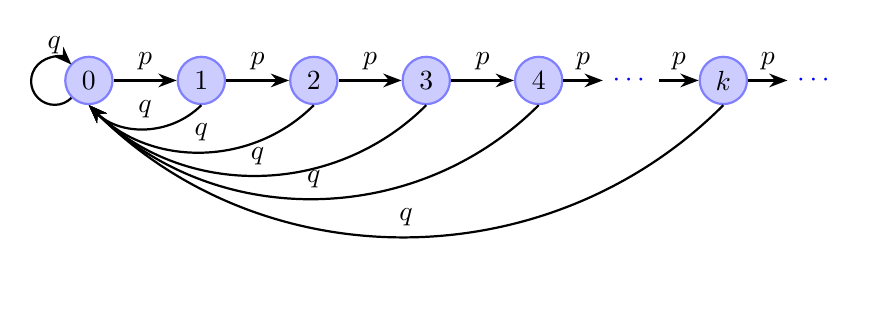
\begin{tikzpicture}
			[%%%%%%%%%%%%%%%%%%%%%%%%%%%%%%%%%%%%%%%%%%%%%%%%%%%%%%%%%%
				node distance =.8cm,>=Stealth,
				place/.style={circle,draw=blue!50,fill=blue!20,thick,
							  inner sep=0pt,minimum size=6mm},
				dotsstyle/.style={text=blue}
			]%%%%%%%%%%%%%%%%%%%%%%%%%%%%%%%%%%%%%%%%%%%%%%%%%%%%%%%%%%
			\node[place] (0) {$0$};
			\node[place] (1) [right=of 0] {$1$};
			\node[place] (2) [right=of 1] {$2$};
			\node[place] (3) [right=of 2] {$3$};
			\node[place] (4) [right=of 3] {$4$};
			\node[dotsstyle] (dots1) [node distance=0.5cm,right=of 4] {$\cdots $};
			\node[place] (k) [node distance=0.5cm,right=of dots1] {$k$};
			\node[dotsstyle] (dots2) [node distance=0.5cm,right= of k] {$\cdots $};

			\draw [->,thick] (0.south west) arc (-45:-315:0.3) node [above left] {$q$};
			
			\foreach \i in {0,1,2,3}
				\draw [->,thick] (\i.east) to node[above] {$p$}({\the\numexpr\i+1}.west);

			\draw [->,thick] (4.east) to node[above] {$p$} (dots1.west);
			\draw [->,thick] (dots1.east) to node[above] {$p$} (k.west);
			\draw [->,thick] (k.east) to node[above] {$p$} (dots2.west);
			
			\foreach \i in {1,2,3,4}
				\draw [->,thick] (\i.south) to [bend left=45] node[above] {$q$} (0.south);

			\draw [->,thick] (k.south) to [bend left=45] node[above] {$q$} (0.south);
		\end{tikzpicture}
		\caption{3.12图解}
	\end{figure}
\end{solution}

\begin{problem}{3.13}
	试证各方向游动的概率相等的对称随机游动在二维时是常返的, 而在三维时却是瞬过的.
	\\ (此处答案仅给出二维情况,三维情况不是作业要求(逃))
\end{problem}
\begin{solution}[1(jkadbear及郑老师解法)]
	设$\{X_n,n\geqslant 0\}$为二维对称随机游动,其状态空间为二维实平面上所有的整数点(格点),易知该M.C.为不可约的,故仅需考虑状态0(原点$(0,0)$)的常返性,且仅需考虑$P_{00}^{(2n)}$.
	\[\begin{split}
		P_{00}^{(2n)} & = \sum_{k=0}^{n}\frac{(2n)!}{k!k!(n-k)!(n-k)!}\left(\frac{1}{4}\right)^{2n} = \left(\frac{1}{4}\right)^{2n}\sum_{k=0}^{n}\binom{2n}{n}\binom{n}{k}^{2} \\ 
		& = \left(\frac{1}{4}\right)^{2n}\binom{2n}{n}\underbrace{\sum_{k=0}^{n}\binom{n}{k}\binom{n}{n-k}}_{=\binom{2n}{n}}\\
		& = \left(\frac{1}{4}\right)^{2n}\binom{2n}{n}^{2} = \left(\frac{1}{4}\right)^{2n}\left[\frac{(2n)!}{(n!)^2}\right]^2 \xrightarrow{\text{Stirling}}\left(\frac{1}{4}\right)^{2n}\left[\frac{(2n)^{2n+\frac{1}{2}}\e^{-2n}\sqrt{2\uppi}}{n^{2n+1}\e^{-2n}2\uppi}\right]^2\\
		& = \frac{1}{n\uppi}
	\end{split}\]
	而级数$\sum_{n=1}^{\infty}\frac{1}{n\uppi}$发散,故$\sum_{n=1}^{\infty}P_{00}^{(n)}$发散,从而该M.C.为常返的.进一步可以证明$\{X_n,n\geqslant 0\}$为零常返的,且周期为2
\end{solution}
\begin{solution}[2]
	前面大差不差.
	\[\begin{split}
		P_{ii}^{(n)} & = \sum_{k=0}^{n}\binom{2n}{k,k,n-k,n-k}\left(\frac{1}{4}\right)^{2n} = \sum_{k=0}^{n}\frac{(2n)!}{k!k!(n-k)!(n-k)!}\frac{1}{2^{4n}} \\
		& = \sum_{k=0}^{n}\binom{n}{k}\frac{(n+1)\cdots (2n)}{k!(n-k)!}\frac{1}{2^{4n}} = \sum_{k=0}^{n}\binom{n}{k}\frac{(\frac{n+1}{2})(\frac{n+2}{2})\cdots n}{k!(n-k)!}\cdot \frac{1}{2^{3n}}\\
		& > \sum_{k=0}^{n}\binom{n}{k}\frac{n!}{k!(n-k)!}\cdot \frac{1}{2^{3n}}\\
		& =\sum_{k=0}^{n}\binom{n}{k}^{2}\cdot \frac{1}{2^{3n}} > \sum_{k=0}^{n}\binom{n}{k}\cdot \frac{1}{2^{3n}} >\sum_{k=0}^{n}\binom{n}{k}\frac{1}{2^n} = 1
	\end{split}\]
	$\therefore \sum_{n=1}^{\infty}P_{ii}^{(n)}>\sum_{n=1}^{\infty}1 = +\infty \Rightarrow i$为常返的,又因为二维随机游动任意状态互达,故该Markov链常返
\end{solution}

\begin{problem}{3.14}
	某厂对该厂生产的同类产品的三种型号调查顾客的消费习惯. 并把它们归结为Markov链模型. 记顾客消费习惯在 $A, B, C $ 三种型号间的转移概率矩阵分别为下列四种. 请依这些转移阵所提供的信息对厂家提出关于 $A, B$ 两种型号的咨询意见.
	\[
		\begin{split}
		&(1)\begin{pmatrix}
				1 & 0 & 0\\
				0 & 1 & 0\\
				0 & 0 & 0
			\end{pmatrix},\qquad
		(2)\begin{pmatrix}
				0 & \frac{1}{2} & \frac{1}{2}\\
				\frac{1}{2} & 0 & \frac{1}{2}\\
				\frac{1}{2} & \frac{1}{2} & 0
			\end{pmatrix},\\
		&(3)\begin{pmatrix}
				\frac{1}{2} & 0 & \frac{1}{2}\\
				\frac{1}{3} & \frac{1}{3} & \frac{1}{3}\\
				\frac{1}{2} & 0 & \frac{1}{2}
			\end{pmatrix},\qquad
		(4)\begin{pmatrix}
				0 & 1 & 0\\
				0 & 0 & 1\\
				1 & 0 & 0
			\end{pmatrix}.
		\end{split}
	\]
\end{problem}
\begin{solution}
	\begin{enumerate}[label=(\arabic*)]
		\item \begin{enumerate}[label=(\alph*)]
				\item 不是概率转移矩阵, 第三行行和不为$1$.
				\item 郑老师的作业题将此图改为
					  $\bm{P}=
					  \begin{pmatrix}
						1 & 0 & 0\\
						0 & 1 & 0\\
						0 & 0 & 1
					  \end{pmatrix}$
					  相应的解答为:$A,B,C$三个状态均为常返,且均为吸收态,但相互之间不可达.说明三种产品都比较好,顾客流都很稳定,但A与B谁更好一些无法比较;
			  \end{enumerate}
		\item \[
				\bm{P}^2 =
				\begin{pmatrix}
					0 & \frac{1}{2} & \frac{1}{2}\\
					\frac{1}{2} & 0 & \frac{1}{2}\\
					\frac{1}{2} & \frac{1}{2} & 0
				\end{pmatrix}^2 =
				\begin{pmatrix}
				\frac{1}{2} & \frac{1}{4} & \frac{1}{4}\\
				\frac{1}{4} & \frac{1}{2} & \frac{1}{4}\\
				\frac{1}{4} & \frac{1}{4} & \frac{1}{2}\\
				\end{pmatrix}
			  \]
			  $\therefore A,B,C$三状态互通, 所有状态可遍历.\\
			  设$\bm{\pi}=(\pi_A,\pi_B,\pi_C)$为经过长时间后三个产品的市场占有额,则
			  \[
				\begin{cases}
					(\pi_A,\pi_B,\pi_C)
					\begin{pmatrix}
						0 & \frac{1}{2} & \frac{1}{2}\\
						\frac{1}{2} & 0 & \frac{1}{2}\\
						\frac{1}{2} & \frac{1}{2} & 0
					\end{pmatrix} = (\pi_A,\pi_B,\pi_C)\\
					\pi_A+\pi_B+\pi_C = 1
				\end{cases} \Rightarrow
				\pi_A = \pi_B = \pi_C = \frac{1}{3}
			  \]
			  $\therefore$三个品牌竞争力差不多, 可以都生产.但从转移概率矩阵来看,$A,B$都有需要改进之处
		\item 由归纳法可知
			  \[
				\bm{P}^n=
				\begin{pmatrix}
					\frac{1}{2} & 0 & \frac{1}{2}\\
					\frac{1}{2}\big(1-\frac{1}{3^n}\big) & \frac{1}{3^n} & \frac{1}{2}\big(1-\frac{1}{3^n}\big)\\
					\frac{1}{2} & 0 & \frac{1}{2}
				\end{pmatrix}
			  \]
			  可见
			  \[\pi_B = \lim_{n\to \infty} \Big(\frac{1}{3}\Big)^n = 0,\]
			  \[
				\begin{cases}
				(\pi_A, \pi_C)\cdot
					\begin{pmatrix}
						\frac{1}{2} & \frac{1}{2}\\
						\frac{1}{2} & \frac{1}{2}
					\end{pmatrix} = (\pi_A, \pi_C)\\
				\pi_A + \pi_C = 1
				\end{cases} \Rightarrow
				\pi_A = \pi_C = \frac{1}{2}
			  \]
			  $\therefore B$将逐渐淡出市场, 建议停止生产$B$, 扩大对$A$的生产.$A,C$常返,$B$瞬过.$A,B$比较,顾客更倾向于消费$A$,且从长远观点看,顾客消费$B$的可能性将趋于零,市场将由$A,C$二分天下.
		\item $\therefore A,B,C$三状态互通, 所有状态可遍历.
			  \[
				\begin{cases}
				(\pi_A,\pi_B,\pi_C)
				\begin{pmatrix}
					0 & 1 & 0\\
					0 & 0 & 1\\
					1 & 0 & 0
				\end{pmatrix} = (\pi_A,\pi_B,\pi_C)\\
				\pi_A+\pi_B+\pi_C = 1
				\end{cases} \Rightarrow
				\pi_A = \pi_B = \pi_C = \frac{1}{3}
			  \]
			  $\therefore A,B,C$市场占有率相同, 可维持现状.与(2)同
			  \begin{figure}[H]
				\centering
				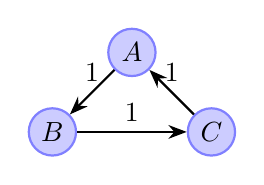
\begin{tikzpicture}
					[%%%%%%%%%%%%%%%%%%%%%%%%%%%%%%%%%%%%%%%%%%%%%%%%%%%%%%%%%%
						node distance =.8cm,>=Stealth,
						place/.style={circle,draw=blue!50,fill=blue!20,thick,
									inner sep=0pt,minimum size=6mm},
						dotsstyle/.style={text=blue}
					]%%%%%%%%%%%%%%%%%%%%%%%%%%%%%%%%%%%%%%%%%%%%%%%%%%%%%%%%%%
					\node[place] (A) {$A$};
					\node[place] (B) [below left=of A] {$B$};
					\node[place] (C) [below right=of A] {$C$};
					
					\draw[->,thick] (A.south west) to node[above]{1} (B.north east);
					\draw[->,thick] (B.east) to node[above]{1} (C.west);
					\draw[->,thick] (C.north west) to node[above]{1} (A.south east);
				\end{tikzpicture}
				\caption{3.14(4)图解}
			  \end{figure}
	\end{enumerate}
\end{solution}

\begin{problem}{3.15}
	考虑一有限状态的Markov链. 试证明
	\begin{enumerate}[label=(\alph*)]
		\item 至少有一个状态是常返的
		\item 任何常返状态必定是正常返的.
	\end{enumerate}
\end{problem}
\begin{solution}[1]
	\begin{enumerate}[label=(\alph*)]
		\item 反设所有状态均为瞬过或零常返(加强结论),则对$\forall i \in S$, 有
			  \[\lim_{n\to +\infty} P^{(n)}_{ii} = 0 \qquad (*)\]
			  考虑$P^{(n)}_{ij} = \sum\limits^{+\infty}_{k=1} f^{(k)}_{ij} P^{(n-k)}_{jj}$, 则有
			  \[\sum^\ell_{k=1} f^{(k)}_{ij} P^{(n-k)}_{jj} \leqslant P^{(n)}_{ij} \leqslant \sum^\ell_{k=1} f^{(k)}_{ij} P^{(n-k)}_{jj} + \sum^{+\infty}_{k=l} f^{(k)}_{ij} \qquad (**)\]
			  固定$\ell$, 令$n\to +\infty$, 则由$(*)$得
			  \[0 \leqslant \lim_{n\to +\infty} P^{(n)}_{ij} \leqslant 0 + \sum^{+\infty}_{k=\ell} f^{(k)}_{ij} \qquad (***)\]
			  在$(***)$中令$\ell \to +\infty$, 由于$\sum\limits^{+\infty}_{k=1} f^{(k)}_{ij} \leqslant 1$收敛
			  \[\therefore \lim_{n\to +\infty} P^{(n)}_{ij} = 0 \qquad (*4)\]
			  若此有限状态$M.C.$有$N$个状态, 则\[\sum^{N}_{j=1} P^{(n)}_{ij} = 1 \qquad (*5)\]
			  $(*5)$中令$n\to +\infty$, 由$(*4)$得$0=1$, 矛盾$\Rightarrow$至少有一个状态是(正)常返的
		\item 若存在零常返状态$i$, 可构造$C(i) = \{j|i\leftrightarrow j\}$,
			  则$C(i)$为原M.C.的一不可约子M.C.(有限状态),
			  于是$C(i)$中所有状态均为零常返, 与有限状态M.C.至少有一个正常返状态矛盾,\\ 
			  $\therefore$任何常返状态均为正常返
	\end{enumerate}
\end{solution}
\begin{solution}[2(郑老师解法)]
	\begin{enumerate}[label=(\alph*)]
		\item 设M.C.的状态空间为$S=\{0,1,2,\cdots ,N\}$.(反证法)若命题为真,则M.C.的所有状态为瞬过的.从而对$\forall i,j\in S$有$\lim_{n \to \infty}P_{ij}^{(n)}=0$,但另一方面又有:
			  \[\sum_{j=0}^{N}P_{ij}^{(n)}=1\qquad (\forall i\in S,n\in \mathbb{N})\]
			  两边取极限得到
			  \[1=\lim_{n \to \infty}\sum_{j=0}^{N}P_{ij}^{(n)} = \sum_{j=0}^{N}\lim_{n \to \infty}P_{ij}^{(n)} = \sum_{j=0}^{N}0 = 0\]
			  矛盾.从而(a)得证
		\item (反证法)若命题不真,则M.C.至少存在一个零常返状态.设$S_1\subseteq S$为全体零常返状态构成的子集,易证$S_1$为闭集.为叙述方便,无妨设$S_1=\{0,1,2,\cdots ,M\}\quad (M\leqslant N)$.则原M.C.限制在$S_1$上仍为一M.C.,从而有:
			  \[\sum_{j\in S_1}P_{ij}[w(n)] = \sum_{j=0}^{M}P_{ij}^{(n)} = 1 \qquad (\forall i\in S_1,n\in \mathbb{N})\qquad (*)\]
			  另一方面,由类似于$(a)$的理由可知,对于$\forall i,j\in S_1$,有$\lim_{n \to \infty}P_{ij}^{(n)} = 0$,从而对(*)式两边取极限得到:
			  \[0 = \lim_{n \to \infty}\sum_{j=1}^{M}P_{ij}^{(n)} = \lim_{n \to \infty}1 = 1\]
			  矛盾.从而该M.C.不可能存在零常返状态.即(b)得证.$\qedhere$
	\end{enumerate}
\end{solution}

\begin{problem}{3.16}
	考虑一生长与灾害模型. 这类Markov链有状态 $0,1,2,\cdots,$ 当过程处于状态$i$时它既可能以概率$p_i$转移到$i+1$(生长)也能以概率$q_i = 1 - p_i$ 落回到状态$0$(灾害). 而从状态“0”又必然“无中”生有. 即$P_{01} \equiv 1$.
	\begin{enumerate}[label=(\alph*)]
		\item 试证所有状态为常返的条件是\[\lim_{n\to \infty}(p_1p_2p_3\cdots p_n) = 0.\]
		\item 若此链为常返, 试求其为零常返的条件.
	\end{enumerate}
\end{problem}
\begin{solution}[1]
	\begin{enumerate}[label=(\alph*)]
		\item 其概率转移阵为
			  \[
				\bm{P} =
				\bordermatrix{
					~ & 0   & 1 & 2   & 3   & \cdots \cr
					0 & 0   & 1 & 0   & 0   & \cdots \cr
					1 & q_1 & 0 & p_1 & 0   & ~ \cr
					2 & q_2 & 0 & 0   & p_2 & ~ \cr
					3 & q_3 & 0 & 0   & 0 ~ \cr
					\vdots & \vdots & ~ & ~ & ~ & \ddots \cr
				}
			  \]
			  易知此M.C.不可约, $\therefore$只需证状态$0$常返$\Leftrightarrow~\lim\limits_{n\to +\infty}p_1 p_2\cdots p_n = 0$\\
			  显然$f^{(0)}_{00} = f^{(1)}_{00} = 0, f^{(2)}_{00} = q_1$
			  \[
				\begin{split}
					\bm{f^{(n)}_{00}} & =
					\begin{pmatrix}
						1 & 0 & 0 & \cdots
					\end{pmatrix}
					\begin{pmatrix}
						0 & p_1 & 0 & 0 & \cdots\\
						0 & 0 & p_2 & 0 & \cdots\\
						0 & 0 & 0 & p_3 & \cdots\\
						\vdots & \vdots & \vdots & \vdots & \ddots
					\end{pmatrix}^{n-2}
					\begin{pmatrix}
						q_1\\
						q_2\\
						q_3\\
						\vdots
					\end{pmatrix}\\
					& = \bm{A}\bm{B}^{n-2}\bm{C}^T, \quad (n\geqslant 3)
				\end{split}
			  \]
			  易知
			  \[
				\bm{B}^{n-2} =
				\begin{pmatrix}
					\underbrace{\begin{matrix}0 & \cdots & 0 \end{matrix}}_{n-2\text{个}} & p_1\cdots p_{n-2} & 0 & \cdots \\
					\underbrace{\begin{matrix}0 & \cdots & 0 \end{matrix}}_{n-2\text{个}} & 0 & p_2\cdots p_{n-2} & \cdots \\
					\vdots & \vdots & \vdots & \ddots
				\end{pmatrix}
			  \]
			  \[\therefore f^{(n)}_{00} = (\,\overbrace{0\,\cdots\,0}^{n-2\text{个}}\,p_1\cdots p_{n-2}\,0\,0\,\cdots)(q_1\,q_2\,\cdots)^T = p_1\cdots p_{n-2}q_{n-1}\]
			  \[
				\begin{split}
					\therefore f_{00} & = q_1 + \sum^{+\infty}_{n=3}p_1\cdots p_{n-2}q_{n-1}\\
					& = 1 - p_1 + \sum^{+\infty}_{n=3}(p_1\cdots p_{n-2} - p_1\cdots p_{n-2}p_{n-1})\\
					& = 1 - \lim_{n\to +\infty}p_1 p_2\cdots p_n
				\end{split}
			  \]
			  而状态$0$常返$\Leftrightarrow f_{00} = 1 \Leftrightarrow \lim\limits_{n\to +\infty}p_1 p_2\cdots p_n = 0$.
		\item 只需考虑状态$0$,
			  \[
				\begin{split}
					\mu_0 & = \sum^{+\infty}_{n=0}nf^{(n)}_{00}\\
					& = 2(1-p_1)+\sum^{+\infty}_{n=3}n(p_1\cdots p_{n-2} - p_1 \cdots p_{n-1})\\
					& = 2 + p_1 + p_1 p_2 + p_1 p_2 p_3 + \cdots
				\end{split}
			  \]
			  若为零常返, 则$\mu_0 = +\infty \Leftrightarrow $级数$\sum\limits^{+\infty}_{n=1}p_1\cdots p_n$发散(且通项趋于$0$)
	\end{enumerate}
\end{solution}
\begin{solution}[2(郑老师解法)]
	该M.C.的状态转移图可画出:
	\begin{figure}[H]
		\centering
		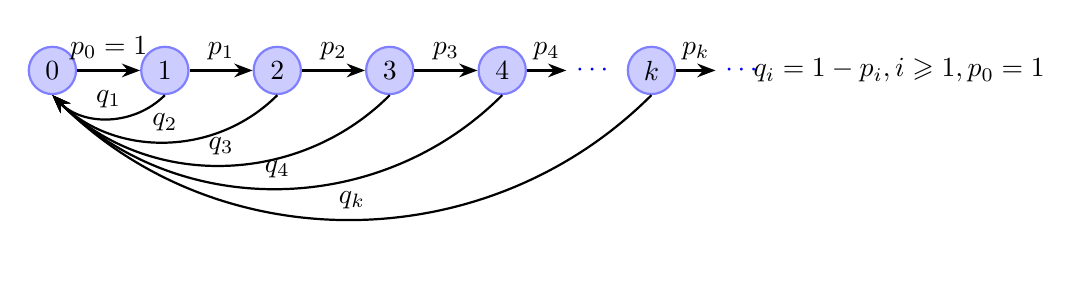
\begin{tikzpicture}
			[%%%%%%%%%%%%%%%%%%%%%%%%%%%%%%%%%%%%%%%%%%%%%%%%%%%%%%%%%%
				node distance =.8cm,>=Stealth,
				place/.style={circle,draw=blue!50,fill=blue!20,thick,
							  inner sep=0pt,minimum size=6mm},
				dotsstyle/.style={text=blue}
			]%%%%%%%%%%%%%%%%%%%%%%%%%%%%%%%%%%%%%%%%%%%%%%%%%%%%%%%%%%
			\node[place] (0) {$0$};
			\node[place] (1) [right=of 0] {$1$};
			\node[place] (2) [right=of 1] {$2$};
			\node[place] (3) [right=of 2] {$3$};
			\node[place] (4) [right=of 3] {$4$};
			\node[dotsstyle] (dots1) [node distance=0.5cm,right=of 4] {$\cdots $};
			\node[place] (k) [node distance=0.05cm,right=of dots1] {$k$};
			\node[dotsstyle] (dots2) [node distance=0.5cm,right=of k] {$\cdots $};
			
			\foreach \i in {1,2,3}
				\draw [->,thick] (\i.east) to node[above] {$p_{\i}$}({\the\numexpr\i+1}.west);
			
			\draw [->,thick] (0.east) to node[above] {$p_0=1$} (1.west);


			\draw [->,thick] (4.east) to node[above] {$p_4$} (dots1.west);
			\draw [->,thick] (k.east) to node[above] {$p_{k}$} (dots2.west);
			
			\foreach \i in {1,2,3,4}
				\draw [->,thick] (\i.south) to [bend left=45] node[above] {$q_{\i}$} (0.south);

			\draw [->,thick] (k.south) to [bend left=45] node[above] {$q_k$} (0.south);
			\draw (dots2) node [right] {$q_i=1-p_i,i\geqslant 1,p_0=1$};
		\end{tikzpicture}
		\caption{3.16图解}
	\end{figure}
	\begin{enumerate}[label=(\alph*)]
		\item 由上图易知M.C.为不可约,非周期的.又:
			  \[f_{00}^{(1)}=0, f_{00}^{(2)}=q_1=1-p_1, f_{00}^{(3)}=p_1(1-p_2), \cdots ,f_{00}^{(n)}=p_1p_2\cdots p_{n-2}(1-p_{n-1})\]
			  从而\[f_{00}^{(n)} = \sum_{n=2}^{\infty}p_1p_2\cdots p_{n-2}(1-p_{n-1} = \lim_{n \to \infty}(1-p_1 p_2 \cdots p_n))\]
			  故0及所有状态为常返$\Longleftrightarrow \lim\limits_{n\to \infty}p_1 p_2 \cdots p_n = 0$
		\item 求解线性方程组$\displaystyle \bm{\pi} = \bm{\pi}\bm{P},\quad \sum_{j=0}^{\infty}\pi _j = 1$解得:
			  \[
				\begin{cases}
					\pi_1 & = \pi_0\\
					\pi_2 & = p_1 \pi_0\\
					& \vdots\\
					\pi_n & = p_1 p_2 \cdots p_{n-1}\pi_0 
				\end{cases}\quad \text{且}\quad
				\pi_0 = \frac{1}{2+\sum_{n=1}^{\infty}p_1 p_2 \cdots p_n}
				\quad \text{故:}
			  \]
			  \begin{itemize}
				\item 当$\sum_{n=1}^{\infty}p_1 p_2 \cdots p_n < +\infty$时,平稳分布$\bm{\pi}$存在,此时M.C.为正常返,亦即为不可约遍历.
				\item 当$\sum_{n=1}^{\infty}p_1 p_2 \cdots p_n = +\infty$但$\lim\limits_{n\to \infty}p_1 p_2 \cdots p_n = 0$时,正常返
				\item 当$\lim\limits_{n\to \infty}p_1 p_2 \cdots p_n = p > 0$时,M.C.为瞬过的.
			  \end{itemize}
			  亦可直接计算$\mu_0 = \sum_{n=1}^{\infty}nf_{00}^{(n)} = \sum_{n=2}^{\infty}np_1 p_2 \cdots p_{n-2}(1-p_{n-1}) = 2+\sum_{n=1}^{\infty}p_1 p_2 \cdots p_n$,从而得出同上的结论
	\end{enumerate}
\end{solution}

\begin{problem}{3.17}
	试计算转移概率阵
	\[
		\bm{P} =
		\begin{pmatrix}
			\frac{1}{2} & \frac{1}{2} & 0\\
			\frac{1}{3} & \frac{1}{3} & \frac{1}{3}\\
			\frac{1}{6} & \frac{1}{2} & \frac{1}{3}
		\end{pmatrix}
	\]
	的极限分布.
\end{problem}
\begin{solution}
	设$\bm{\pi}$为该M.C.的平稳分布, $\bm{\pi}= (\pi_0, \pi_1, \pi_2)$\\
	\[
		\begin{cases}
			\pi \geqslant 0\\
			\sum\limits^2_{i=0} \pi_i = 1\\
			\bm{\pi}\bm{P} = \bm{\pi}
		\end{cases}\Rightarrow
		\bm{\pi} = \left(\frac{5}{14}, \frac{6}{14}, \frac{3}{14}\right)
	\]
	易知该M.C.不可约且遍历\quad $\therefore$ 极限分布为
	$
	\begin{pmatrix}
		\frac{5}{14} & \frac{6}{14} & \frac{3}{14}\\
		\frac{5}{14} & \frac{6}{14} & \frac{3}{14}\\
		\frac{5}{14} & \frac{6}{14} & \frac{3}{14}
	\end{pmatrix}
	$
\end{solution}

\begin{problem}{3.18}
	假定在逐日的天气变化模型中, 每天的阴晴与前两天的状况关系很大. 于是可考虑$4$状态的Markov链:接连两晴天, 一晴一阴, 一阴一晴, 以及接连两阴天, 分别记为$(S, S), (S, C), (C, S), (C, C)$. 该链的转移概率阵为
	\[\bm{P} =
		\bordermatrix{
		~ & (S,S) & (S,C) & (C,S) & (C,C) \cr
		(S,S) & 0.8 & 0.2 & 0 & 0 \cr
		(S,C) & 0 & 0 & 0.4 & 0.6 \cr
		(C,S) & 0.6 & 0.4 & 0 & 0 \cr
		(C,C) & 0 & 0 & 0.1 & 0.9 \cr}
	\]
	试求这一Markov链的平稳分布. 并求出长期平均的晴朗天数.
\end{problem}
\begin{solution}
	设其平稳分布为$\bm{\pi}= (\pi_0, \pi_1, \pi_2, \pi_3)$\\
	\[
		\begin{cases}
			\pi \geqslant 0\\
			\sum\limits^3_{i=0} \pi_i = 1\\
			\bm{\pi}\bm{P} = \bm{\pi}
		\end{cases} \Rightarrow
    \bm{\pi} = \left(\frac{3}{11}, \frac{1}{11}, \frac{1}{11}, \frac{6}{11}\right)
	\]
	$\bm{\pi}$反映了M.C.中各状态在长期中所占的平均比例\\
	$\therefore$一年中晴朗的天数 $ = \frac{365}{2} \times \left(\frac{3}{11} \times 2 + \frac{1}{11} + \frac{1}{11}\right) = 365\times \frac{4}{11} = 132.7$(天)
\end{solution}

\begin{problem}{3.19}
	某人有$M$把伞并在办公室和家之间往返. 如某天他在家时(办公室时)下雨了而且家中(办公室)有伞他就带一把伞去上班(回家), 不下雨时他从不带伞. 如果每天与以往独立地早上(或晚上)下雨的概率为$p$, 试定义一$M+1$状态的Markov链以研究他被雨淋湿的机会.
\end{problem}
\begin{solution}
	定义$X_n$:第$n$天早晨家中雨伞数, $\therefore \{X_n, n \geqslant 0\}$为一M.C.,令$q=1-p$,可得转移概率矩阵为:
	\[
		\bm{P} =
		\bordermatrix{
			~ & 0 & 1 & 2 & \cdots & M\!-\!1 & M & M\!+\!1 \cr
			0 & q & p & 0 & ~ & ~ & ~ & ~\cr
			1 & pq & p^2\!+\!q^2 & pq & ~ & ~ & ~ & ~\cr
			2 & 0 & pq & p^2\!+\!q^2 & ~ & ~ & ~ & ~\cr
			\vdots & ~ & ~ & ~ & \ddots & ~ & ~ & ~\cr
			M\!-\!1 & ~ & ~ & ~ & ~ & pq & p^2\!+\!q^2 & pq\cr
			M & ~ & ~ & ~ & ~ & 0 & pq & q^2\cr}
	\]
	由状态转移图易知M.C.为不可约遍历的,求其平稳分布(极限分布)为:
	设$\bm{\pi}= (\pi_0, \pi_1, \cdots, \pi_M)$为其平稳分布
	\[
		\begin{cases}
			\pi \geqslant 0\\
			\sum\limits^M_{i=0}\pi_i = 1\\
			\bm{\pi}\bm{P} = \bm{\pi}
		\end{cases} \Rightarrow
		\begin{cases}
			\pi_0 = \frac{1-p}{M+1-p}\\
			\pi_i = \frac{1}{M+1-p} (i = 1,2,\cdots,M)
		\end{cases}
	\]
易知此M.C.遍历, \\
$\therefore \pi$又是其极限分布, 其被雨淋湿的概率为
\[
P_{\text{淋}} = p\pi_0+p(1-p)\pi_M = 2p\frac{1-p}{M+1-p}
\]
\end{solution}

下面几道题涉及分支过程,这部分没讲,故都没写.

\begin{problem}{3.20}
	血液培养在时刻0从一个红细胞开始,一分钟之后红细胞死亡可能出现下面几种情况:以1/4再生2个红细胞,以1/2的概率再生1个红细胞和1个白细胞,也有1/4的概率产生2个白细胞.再过一分钟后每个红细胞以同样的规律再生下一代而白细胞则不再生.并假定每个细胞的行为是独立的.
	\begin{enumerate}[label=(\alph*)]
		\item 从培养开始$n+1$分钟不出现白细胞的概率是多少?
		\item 整个培养过程停止的概率是多少?
	\end{enumerate}
\end{problem}
\begin{solution}
	\begin{enumerate}[label=(\alph*)]
		\item $p=\frac{1}{4}\left(\frac{1}{4}\right)^2 \cdots \left(\frac{1}{4}\right)^{2^n}\left(\frac{1}{4}\right)^{2^{n+1}-1}$
			  \begin{itemize}
				\item 时刻 0 1 ... $n$
				\item 个数 1 2 ... $2^n$
			  \end{itemize}
		\item \textcolor{blue}{法一:}\\
			  \[\Phi(s) = \sum_{k=0}^{\infty}p_k s^k = \frac{1}{4}s^0 +\frac{1}{2}s^1 + \frac{1}{4}s^2\]
			  \[\Phi(s)=s\quad \frac{1}{4}s^2 - \frac{1}{2}s + \frac{1}{4} = 0\Rightarrow s=1 \Rightarrow P_{\text{消亡}}=1\]
			  \textcolor{blue}{法二:}\\
			  \[\E(Z_1)=\frac{1}{2}+2\cdot \frac{1}{4}=1=\mu \Rightarrow P_{\text{消亡}}=1\]
	\end{enumerate}
\end{solution}

\begin{problem}{3.21}
	分支过程中一个体产生后代的分布为$p_0=q,p_1=p \quad (p+q=1)$,试求第$n$代总体的均值和方差及群体消亡的概率.如产生后代的分布为$p_0=1/8,p_1=1/2,p_2=1/4,p_3=1/8$,试回答同样的问题.
\end{problem}
\begin{solution}
	\begin{enumerate}[label=(\roman*)]
		\item $p_0=q, p_1=p$\\
			  $Z_1$为第1代第1个个体的后代,$\p(Z_1=k)=p_k, \E(Z_1)=\mu, \var(Z_1)=\sigma ^2$
			  \[\begin{split}
				\E(X_{n+1}) &= \mu ^{n+1}\\
				\var(X_{n+1}) &= \begin{cases}
					\sigma ^2 \mu ^n \frac{1-\mu ^{n+1}}{1-\mu},& \mu \neq 1\\
					(n+1)\sigma ^2, & \mu = 1
				\end{cases}
			  \end{split}\]
			  故$\mu = \E(Z_1) = p \Rightarrow \E(X_n)=p^n$\\
			  $\var(Z_1)=pq=\sigma ^2\Rightarrow \var(X_n)=\begin{cases}
				pq\cdot p^{n-1}\cdot \frac{1-p^n}{1-p}=p^n(1-p^n),& p\neq 1\\
				0, & p=1
			  \end{cases}$
			  $\Phi(s)= p_{01}p_1 s\Rightarrow \Phi(s)=s\Rightarrow 1-p=(1-p)s$\\
			  $p\neq 1\Rightarrow \pi=1 \quad p=1,X_n=1,\pi=0$
		\item $p_0=\frac{1}{8},p_1=\frac{1}{2},p_2=\frac{1}{4},p_3=\frac{1}{8}\Rightarrow \E(Z_1)=\frac{11}{8},\quad \var(Z_1)=\frac{47}{64}$\\
			  $\Rightarrow \E(X_n)=\left(\frac{11}{8}\right)^n,\quad \var(X_n)=\frac{47}{64}\left(\frac{11}{8}\right)^{n-1} = \frac{47}{24}\left(\frac{11}{8}\right)^{n-1}\left[1-\left(\frac{11}{8}\right)^n\right]$\\
			  $\Phi(s)=s\Rightarrow s=1\text{或}\frac{-3\pm\sqrt{13}}{2}\Rightarrow \pi = \frac{-3+\sqrt{13}}{2}$
	\end{enumerate}
\end{solution}

\begin{problem}{3.22}
	若单一个体产生后代的分布为$p_0=q, p_1=p\quad (p+q=1)$,并假定过程开始时的祖先数为1,试求分支过程第3代总数的分布.
\end{problem}
\begin{solution}
	由题意得,$\p(X_n=1)=p^n,\p(X_n=0)=1-p^n$\\
	$\therefore \p(X_3=1)=p^3,\p(X_3=0)=1-p^3$
\end{solution}

\begin{problem}{3.23}
	一连续时间Markov链有$0$和$1$两个状态, 在状态$0$和$1$的逗留时间服从参数为$\lambda > 0$及$\mu > 0$的指数分布. 试求在时刻$0$从状态$0$起始, $t$时刻后过程处于状态$0$的概率$P_{00}(t)$
\end{problem}
\begin{solution}
	\[
		\begin{split}
			P_{00}(t+h) & = \sum^{}_{k \geqslant 0} P_{0k}(t)P_{k0}(h)\\
			& = P_{00}(t)P_{00}(h) + P_{01}(t)P_{10}(h)\\
			& = P_{00}(1-\lambda h + o(h))+(1-P_{00}(t))(\mu h + o(h))
		\end{split}
	\]
	$\displaystyle \therefore \frac{P_{00}(t+h) - P_{00}(t)}{h} = -(\lambda + \mu) P_{00}(t) + \mu + \frac{o(h)}{h}$\\
	令$h\to 0$, 则$P'_{00}(t) = -(\lambda + \mu) P_{00}(t) + \mu$\\
	而$P_{00}(0) = 1$, 解微分方程得
	\[P_{00}(t) = \frac{\lambda}{\lambda + \mu}\e^{-(\lambda + \mu)t} + \frac{\mu}{\lambda + \mu}\]
\end{solution}

\begin{problem}{3.24}
	在第23题中如果$\lambda = \mu$. 定义$N(t)$为过程在$[0,t]$中改变的次数, 试求$N(t)$的概率分布.
\end{problem}
\begin{solution}
	设$f(t)$为状态$0$(或$1$)逗留时间的概率密度函数, $f(t) = \lambda \e^{-\lambda t}$\\
	记$P_k(t) = \p[N(t) = k | N(0) = 0 ],\quad (k = 0,1,2,\cdots)$
	\[
		\begin{split}
			P_0(t) & = \p(\text{在状态$0$(或$1$)逗留时间$t_s > t$})\\
			& = 1 - \p(t_s \leqslant t)\\
			& = 1-\int^t_0 \lambda \e^{\lambda t_s}\d t_s\\
			& = \e^{-\lambda t}
		\end{split}
	\]
	猜想$P_k(t) = \frac{(\lambda t)^k}{k!} \e^{-\lambda t}$\\
	设到$k-1$为止猜想成立, 则
	\[
		\begin{split}
			P_k(t) & = \int^t_0 f(t_s)P_{k-1}(t-t_s)\d t_s\\
			& = \int^t_0 \lambda \e^{-\lambda t_s} \frac{[\lambda(t-t_s)]^{k-1}}{(k-1)!} \e^{-\lambda(t-t_s)}\d t_s\\
			& = \frac{{\lambda}^k}{(k-1)!} \e^{-\lambda t}\int^t_0(t-t_s)^{k-1}\d t_s\\
			& = \frac{(\lambda t)^k}{k!}\e^{-\lambda t}
		\end{split}
	\]
	综上, 当$\lambda = \mu$时$N(t)$服从参数为$\lambda t$的Possion分布
\end{solution}

\begin{problem}{3.25}
	记$X(t)$为纯生过程,且有
	\[
		\begin{aligned}
			\p[X(t+h)-X(t)=1|X(t)\text{为奇数}] & = \alpha h + o(h)\\
			\p[X(t+h)-X(t)=1|X(t)\text{为偶数}] & = \beta h + o(h)
		\end{aligned}
	\]
	及$X(0)=0$,试分别求事件"$X(t)$为偶数"及"$X(t)$为奇数"的概率.
\end{problem}
\begin{solution}
	本题暂缺
\end{solution}

\begin{problem}{3.26}
	考虑状态$0,1,\cdots,N$上的纯生过程$X(t)$, 假定$X(0)=0$以及$\lambda_k = (N-k)\lambda, k = 0,1,\cdots,N$. 其中$\lambda_k$满足
	\[P\{X(t+h) - X(t) = 1 | X(t) = k\} = \lambda_k h + o(h),\]
	试求$P_n(t) = P(X(t) = n)$, 这是新生率受群体总数反馈作用的例子.
\end{problem}
\begin{solution}
	本题暂缺
\end{solution}

\begin{problem}{3.27}
	在某化学反应中,由分子$A$与$B$发生反应而产生分子$C$.假定在很小时间$h$之内一个分子$A$与$B$接近能发生化学反应的概率与$h$及$A,B$当前的分子数成正比.假定在反应开始时$A,B$分子数相同,并记过程$X(t)$为$A$分子在时刻$t$的数目.试建立其随机过程模型.
\end{problem}
\begin{solution}
	本题暂缺
\end{solution}

\begin{problem}{3.28}
	有无穷多个服务员的排队系统. 假定顾客以参数为$\lambda$的Possion过程到达, 而服务员的数量巨大, 可理想化为无穷多个. 顾客一到就与别的顾客相独立地接受服务, 并在时间$h$内完成服务的概率近似为$\alpha h$. 记$X(t)$为在时刻$t$正接受服务的顾客总数, 试建立此过程的转移机制的模型.
\end{problem}
\begin{solution}
	本题暂缺
\end{solution}

\begin{problem}{3.29}
	一个由$N$个部件组成 的循环装置.从$C_1,C_2,\cdots $到$C_N$顺时针排列.第$k$个部件会持续工作一段时间,其分布是以$\lambda _k$为参数的指数分布.一旦它停止工作,顺时针方向的下一个元件就立即接替它开始运行.假定各部件及同一部件的不同次运行都是相互独立的.记$X(t)$为时刻$t$正在运行的部件的序号.试写出模型及转移概率所满足的微分方程.当$N=2,\lambda_1=\lambda_2=1$.初始状态为1时试求解$P_{11}(t)$及$P_{12}(t)$.
\end{problem}
\begin{solution}
	本题暂缺
\end{solution}

\begin{problem}{3.30}
	试写出纯生过程的Kolmogorov向前微分方程. 在初始条件$P_{ii}(0) = 1$下试写出$P_{ii}(t)$及$P_{ij}(t)$应满足的方程. 特别对$\lambda_j = j\lambda$的Yule过程求出$P_{ij}(t)$的明显表达式.
\end{problem}
\begin{solution}
	本题暂缺
\end{solution}

\begin{problem}{3.31}
	两个通讯卫星放入轨道. 每一个卫星的工作寿命都是以$\mu$为参数的指数分布. 一旦失效就再放射一颗新卫星替换它. 所需的准备及发射时间服从以$\lambda$为参数的指数分布. 记$X(t)$为时刻$t$时在轨道中工作的卫星数. 假定这是一个状态空间为$\{0,1,2\}$的连续时间Markov链模型. 试建立Kolmogorov向前及向后微分方程.
\end{problem}
\begin{solution}
	本题暂缺
\end{solution}

\clearpage
\section{第四章~平稳过程}
\noindent\textcolor{red}{以下如果没有指明变量$t$的取值范围,一般视为$t\in \mathbb{R}$,平稳过程是指宽平稳过程.}

\begin{problem}{4.1}
	设$X(t)=\sin Ut$,这里$U$为$(0,2\uppi)$上的均匀分布.
	\begin{enumerate}[label=(\alph*)]
		\item 若$t=1,2,\cdots$,证明$\{X(t),t=1,2,\cdots \}$是宽平稳但不是严平稳过程,
		\item 设$t\in [0,+\infty )$,证明$\{X(t),t\geqslant 0\}$既不是严平稳也不是宽平稳过程.
	\end{enumerate}
\end{problem}
\begin{solution}
	\begin{enumerate}[label=(\alph*)]
		\item \[\E[X(t)] = \E(\sin Ut) = \int^{2\uppi}_0 \frac{1}{2\uppi}\sin Ut \d U = 0 \qquad (t = 1,2,\cdots)\]
			  \[
				\begin{split}
				\cov(X(t), X(s)) & = \E(\sin Ut \cdot \sin Us)\\
								& = \frac{1}{2}\E\left[\cos(t-s)U-\cos(t+s)U\right]\\
								& = \frac{1}{4\uppi}\left\{\frac{1}{t-s}\sin(t-s)U \Big|^{2\uppi}_0 - \frac{1}{t+s}\sin(t+s)U \Big|^{2\uppi}_0\right\}\\
								& = 0 \qquad (t\neq s)
				\end{split}
			  \]
			  当$t=s$时$\cov(X(t), X(s)) = \E(\sin^2 Ut) = \frac{1}{2}$ \quad $\therefore$ 是宽平稳\\
			  考虑$F_t(x) = \p(\sin Ut \leqslant x)$, 显然$F_{t+h} = \p[\sin U(t+h) \leqslant x]$与其不一定相同 \quad $\therefore$ 不是严平稳
		\item \[\E[X(t)] = \frac{1}{2\uppi t}(1-\cos 2\uppi t)\]
			  \[D[X(t)] = \E\left(\sin Ut - \frac{1}{2\uppi t}(1-\cos 2\uppi t)\right)^2 = \frac{1}{2} - \frac{\sin 4\uppi t}{8\uppi t} - \left(\frac{1-\cos 2\uppi t}{2\uppi t}\right)^2\]
			  都与$t$相关 \quad $\therefore$ 不是宽平稳\\
			  若其严平稳, 则因二阶矩存在, 应为宽平稳, 矛盾.\quad $\therefore$ 不是严平稳.\\
	\end{enumerate}
\end{solution}

\begin{problem}{4.2}
	设$\{X_n, n = 0,1,2\cdots\}$ 是平稳序列, 定义$\{X^{(i)}_n, n = 1,2,\cdots\}, i = 1, 2, \cdots, $为
	\[\begin{aligned}
		X^{(1)}_n &  = X_n - X_{n-1},\\
		X^{(2)}_n & = X^{(1)}_n - X^{(1)}_{n-1},\\
		& \cdots\cdots
	\end{aligned}
	\]
	证明这些序列仍是平稳序列.\\
\end{problem}
\begin{solution}
	\begin{enumerate}[label=$\arabic*^\circ$]
		\item $\ell = 0$时,$\E(X_n)$依定义为常数$C_0$\\
		      $\cov(X_n, X_m)$依定义为$n-m$的函数$f_0(n-m)\Rightarrow$ 成立
		\item 设当$\ell \leqslant k$时成立, 则当$\ell = k + 1$时
			  \[\E X^{(\ell)}_n = \E(X^{(k)}_n - X^{(k)}_{n-1}) = C_k - C_k = 0\]
			  \[
				\begin{split}
					\cov(X^{(k+1)}, X^{(k+1)}_m) & = \E(X^{(k+1)}_n X^{(k+1)}_m)\\
					& = \E\left[(X^{(k)}_n - X^{(k)}_{n-1})(X^{(k)}_m - X^{(k)}_{m-1})\right]\\
					& = \E(X^{(k)}_n X^{(k)}_m) - \E(X^{(k)}_{n-1}X^{(k)}_m) - \E(X^{(k)}_{n}X^{(k)}_{m-1}) + \E(X^{(k)}_{n-1}X^{(k)}_{m-1})\\
					& = f_k(n-m) - f_k(n-1-m) - f_k(n-m+1) + f_k(n-m)\\
					& = f_{\ell}(n-m)
			    \end{split}
			  \]
			只与$n-m$有关\quad $\therefore$是平稳的
	\end{enumerate}
\end{solution}

\begin{problem}{4.3}
	设$X_n = \sum\limits^N_{k=1}\sigma_k\sqrt{2}\cos(a_kn-U_k)$, 这里$\sigma_k$和$a_k$为正常数, $k=1, \cdots, N;U_1, \cdots, U_n$是$(0,2\uppi)$上独立均匀分布随机变量, 证明$\{X_n, n = 0, \pm 1, \cdots\}$是平稳过程.
\end{problem}
\begin{solution}
	\[
		\begin{split}
			\E(X_n) & = \E\left[\sum^N_{k=1}\sigma_k\sqrt{2}(\cos a_k n \cos U_k +\sin a_k n \sin U_k)\right] = 0\\
			& = \sum_{k=1}^{N}a_k \sqrt{2}\big[\E(\cos U_k)\cos a_k n + \E(\sin U_k)\sin a_k n\big]\\
			& = 0\\
			\cov(X_n, X_m) & = \E(X_n, X_m)\\
			& = \E\left[\sum^N_{k=1}\sigma_k\sqrt{2}\cos a_kn-U_k\sum^N_{j=1}\sigma_j\sqrt{2}\cos (a_jm-U_j)\right]\\
			& = \sum^N_{k=1}2\sigma^2_k\E\left[\cos(a_kn-U_k)\cos(a_km-U_k)\right]\\
			& = \sum^N_{k=1}\sigma^2_k\E\left[\cos a_k(n-m) + \cos(a_kn + a_km - 2U_k)\right]\\
			& = \sum^N_{k=1}\sigma^2_k\cos a_k(n-m)\\
		\end{split}
	\]
	只与$n-m$有关\quad $\therefore$宽平稳.
\end{solution}

\begin{problem}{4.4}
	设$A_k, k = 1,2,\cdots,n$是$n$个实随机变量; $\omega_k, k = 1,2,\cdots,n,$是$n$个实数. 试问$A_k$以及$A_k$之间应满足怎样的条件才能使
	\[Z(t) = \sum^n_{k=1}A_k \e^{j\omega_kt}\]
	是一个复的平稳过程.	
\end{problem}
\begin{solution}
	要求
	\[\E[Z(t)] = \sum^n_{k=1}\E (lA_k \e^{j\omega_kt}) = const\]
	$\therefore \E(A_k) = 0$,要求
	\[\cov(Z(t), Z(s)) = \E[Z(t)\overline{Z(s)}] = \sum^{\infty}_{k=1}\sum^{\infty}_{\ell=1}\E(A_k A_\ell)\cdot \e^{j\omega_kt - j\omega_\ell s}\]
	只与$t-s$有关\\
	$\therefore \E(A_k A_l) = 0 \quad (k\neq \ell \text{\,且\,}\omega_k \neq \omega_\ell)$
\end{solution}

\begin{problem}{4.5}
	设$\{X_n, n=1,2,\cdots \}$是一列独立同分布的随机变量序列,$\p(X_n=1)=p,\p(X_n=-1)=1-p,\quad n=1,2,\cdots $,令$S_0=0, S_n=(X_1+\cdots +X_n)/\sqrt{n},\quad n=1,2,\cdots $,求随机序列$\{S_n=1,2,\cdots \}$的协方差函数和自相关函数.$p$取何值时此序列为平稳序列?
\end{problem}
\begin{solution}
	由题意$\E(X_n)=2p-1,\E(X_n^2)=1,\E(S_n)=\frac{1}{\sqrt{n}}\sum_{i=1}^{n}\E(X_1) = \sqrt{n}(2p-1)$
	\begin{enumerate}[label=(\roman*)]
		\item \[\begin{split}
				 & \cov(S_n,S_m) = \E(S_n S_m) = \E(S_n)\E(S_m)\\
				=& \frac{1}{\sqrt{mn}}\sum_{i=1}^{n}\sum_{j=1}^{m}\E(X_i X_j) - \sqrt{mn}(2p-1)^2 \xlongequal{\text{不妨设}m<n} \\
				=& \frac{1}{\sqrt{mn}}\left(\sum_{i=1}^{m}\E(X_i^2)+\sum_{(i,j)=(1,1),i\neq j}^{(i,j)=(m,n)}\E(X_i)\E(X_j)\right) - \sqrt{mn}(2p-1)^2\\
				=& \frac{4m}{\sqrt{mn}}p(1-p)
			  \end{split}\]
		\item \[r_X(n,m)=\E(S_n S_m)=\frac{4\min {m,n}}{\sqrt{mn}}p(1-p)+\sqrt{mn}(2p-1)^2\]
		\item 若$\{S_n\}$平稳,则$\E(S_n)\equiv const$, 由$\sqrt{2}S_n = \sqrt{n}(2p-1) \Rightarrow p=\frac{1}{2}$
			  但此时$\cov(S_n,S_m) = \frac{\min \{m,n\}}{\sqrt{mn}}$与$m,n$有关,故不存在$p$使得序列平稳
	\end{enumerate}
\end{solution}

\begin{problem}{4.6}
	设$\{X(t)\}$是一个平稳过程, 对每个$t \in \mathbb{R}$, $X'(t)$存在. 证明对每个给定的$t$, $X(t)$与$X'(t)$不相关, 其中$X'(t) = \frac{\d X(t)}{\d t}$.
\end{problem}
\begin{solution}
	以下假定求导数和求期望可交换\\
	设$\E[lX(t)] = m, D[X(t)] = \sigma^2$\\
	$\therefore \E(X(t+\Delta t)) = m$\\
	$\because X'(t) = \lim\limits_{\Delta \to 0}\frac{X(t+\Delta t) - X(t)}{\Delta t}$\\
	$\therefore \E(X'(t)) = 0$
	\[
		\begin{split}
			\therefore & \cov(X(t), X'(t))  = \E[X(t)X'(t)] = \frac{1}{2}\E\Big[\big(X^2(t)\big)'\Big] = \frac{1}{2}\big(\E[X^2(t)]\big)'\\
			& = \frac{1}{2}(\sigma^2 + m^2)' = 0
		\end{split}
	\]
	$\therefore$ 不相关
\end{solution}

\begin{problem}{4.7}
	设$\{X(t)\}$是高斯过程, 均值为$0$, 协方差函数$R(\tau) = 4\e^{-2|\tau|}$. 令
	\[Z(t) = X(t+1),\quad W(t) = X(t-1),\]
	\begin{enumerate}[label=(\roman*)]
		\item 求$\E(Z(t)W(t))$和$\E(Z(t) + W(t))^2$;
		\item 求$Z(t)$的密度函数$f_Z(z)$及$\p(Z(t)<1)$;
		\item 求$Z(t), W(t)$的联合密度$f_{Z,W}(z,w)$.
	\end{enumerate}
\end{problem}
\begin{solution}
	\begin{enumerate}[label=(\roman*)]
		\item \[\E[Z(t)W(t)] = \E[X(t+1)X(t-1)] = R(2) = 4\e^{-4}\]
			  \[
				\begin{split}
					\E[Z(t)W(t)]^2 & = \E\big[X^2(t+1)+2X(t+1)X(t-1)+X^2(t-1)\big]\\
								& = 2\E[X^2(t)]+2R(2)\\
								& = 2\big\{D[X(t)]-\E^2[X(t)]\big\} + 4\e^{-4}\\
								& = 2R(0) + 4\e^{-4}\\
								& = 4(1+\e^{-4})
				\end{split}
			  \]
		\item $Z(t) = X(t+1) \sim N(0, 2^2)$
			  \[\begin{aligned}
			  	\therefore f_Z(z) & = \frac{1}{\sqrt{2\uppi \cdot 2^2}}\e^{-\frac{z^2}{2\cdot 2^2}} = \frac{1}{\sqrt{8\uppi}}\e^{-\frac{z^2}{8}}\\
			  	\therefore \p[Z(t)<1] & = \int^1_{-\infty}f_Z(z)\d z = \frac{1}{\sqrt{8\uppi}}\int^1_{-\infty}\e^{-\frac{z^2}{8}}\d z
			  \end{aligned}\]
		\item 显然$f_{Z,W}(z,w)$为二维正态分布概率密度函数,协方差矩阵为
			  \[
				\bm{C} =
				\begin{pmatrix}
					4 & 4\e^{-4}\\
					4\e^{-4} & 4
				\end{pmatrix}
			  \]
			  其逆矩阵
			  \[
				\bm{C}^{-1}=
				\begin{pmatrix}
					\frac{1}{4(1-\e^{-8})} & -\frac{\e^{-4}}{4(1-\e^{-8})}\\
					-\frac{\e^{-4}}{4(1-\e^{-8})} & \frac{1}{4(1-\e^{-8})}
				\end{pmatrix}
			  \]
			  其行列式$\left|\bm{C}\right| = 16(1-\e^{-8})$,期望向量$\bm{\bar{\mu }} = (0,0)$
			  \[
				\begin{split}
					\therefore f_{Z,W}(z,w) & = \frac{1}{2\uppi\left|\bm{C}\right|}\exp\Bigg\{-\frac{1}{2}\Big((z,w)-\bm{\bar{\mu}}\Big)\bm{C}^{-1}\Big((z,w)-\bm{\bar{\mu}}\Big)^T\Bigg\}\\
					& = \frac{1}{8\uppi \sqrt{1-\e^{-8}}}\exp\Bigg\{-\frac{z^2+w^2-2\e^{-4}wz}{8(1-\e^{-8})}\Bigg\}
				\end{split}
			  \]
	\end{enumerate}
\end{solution}

\begin{problem}{4.8}
	设$\{X(t), t\in \mathbf R\}$是一个严平稳过程, $\varepsilon$为只取有限个值的随机变量. 证明$\{Y(t) = X(t-\varepsilon), t\in \mathbf R\}$仍是一个严平稳过程.\\
	提示:对$\varepsilon$用全概率公式.
\end{problem}
\begin{solution}
	设$\varepsilon$可取$\varepsilon_1, \varepsilon_2, \cdots, \varepsilon_n$\\
	\[
		\begin{split}
		\text{则}\, & \p\big\{Y(t_1+h) \leqslant y_1, \cdots, Y(t_k+h) \leqslant y_k\big\}\\
			& = \p\big\{X(t_1-\varepsilon+h) \leqslant y_1, \cdots, X(t_k-\varepsilon+h) \leqslant y_k\big\}\\
			& = \sum^n_{i=1}\p(\varepsilon = \varepsilon_i)\p\big\{X(t_1-\varepsilon_i + h) \leqslant y_1, \cdots, X(t_k-\varepsilon_i + h) \leqslant y_k | \varepsilon = \varepsilon_i\big\}
		\end{split}
	\]
	$\because X(t)$严平稳
	\[
		\begin{split}
		\therefore \text{上式} & = \sum^n_{i=1}\p(\varepsilon = \varepsilon_i)P\big\{X(t_1-\varepsilon_i) \leqslant y_1, \cdots, X(t_k-\varepsilon) \leqslant y_k | \varepsilon = \varepsilon_i\big\}\\
							& = \p\big\{X(t_1-\varepsilon) \leqslant y_1, \cdots, X(t_k-\varepsilon) \leqslant y_k\big\}\\
							& = \p\big\{Y(t_1) \leqslant y_1, \cdots, Y(t_k) \leqslant y_k\big\}\\
		\end{split}
	\]
	$\therefore Y(t)$为严平稳.
\end{solution}

\begin{problem}{4.9}
	设$\{X(t),t\in \mathbb{R}\}$是一个严平稳过程,构造随机过程$Y$如下:$Y(t)=1$,若$X(t)>0;-1,$若$X(t)\leq 0$.证明$\{Y(t),t\in \mathbb{R}\}$是一个平稳过程.如果进一步假定$\{X(t),t\in \mathbb{R}\}$是均值为零的Gauss平稳过程,证明$R_Y(\tau)$为$\frac{2}{\uppi}\arcsin (R_X(\tau)/R_X(0))$.
\end{problem}
\begin{solution}
	本题暂缺.
\end{solution}

\begin{problem}{4.10}
	设$\{X(t)\}$是一个复值平稳过程, 证明
	\[E|X(t+\tau)-X(t)|^2 = 2\Re e(R(0)-R(\tau)).\]
\end{problem}
\begin{solution}
	记$m=\E[X(t)]$
	\[
		\begin{split}
			\text{则} \E\big|X(t+\tau) - X(t)\big|^2 & = \E\big|(X(t+\tau)-m)-(X(t)-m)\big|^2\\
			& = \E\big|X(t+\tau)-m\big|^2 + E\big|X(t)-m\big|^2 - \E\Big[(X(t+\tau)-m)\overline{(X(t)-m)}\,\Big] \\
			& \quad - \E\Big[(X(t)-m)\overline{(X(t+\tau)-m)}\,\Big]\\
			& = 2R(0)-R(-\tau)-R(\tau)
		\end{split}
	\]
	又$\because R(-\tau) = \overline{R(\tau)}$\\
	$\therefore \text{上式} = 2\Re e(R(0)-R(\tau))$
\end{solution}

\begin{problem}{4.11}
	设$\{X(t)\}$是零均值的平稳高斯过程, 协方差函数为$R(\tau)$, 证明
	\[\p(X'(t) \leqslant a) = \phi\Bigg(\frac{a}{\sqrt{-R''(0)}}\Bigg),\]
	其中$\phi(\cdot)$为标准正态分布函数.
\end{problem}
\begin{solution}
	注意到$X'(t)$服从正态分布\\
	而$\E[X'(t)] = \big\{\E[X(t)]\big\}' = 0$\\
	$\var(X'(t)) = \cov(X'(t), X'(t+0)) = -R''(0)$\\
	$\therefore X'(t) \sim N(0,-R''(0))$\\
	\[\therefore \p\big(X'(t) \leqslant a\big) = \p\Bigg(\frac{X'(t)}{\sqrt{-R''(0)}} \leqslant \frac{a}{\sqrt{-R''(0)}}\Bigg) = \phi\Bigg(\frac{a}{\sqrt{-R''(0)}}\Bigg)\]
\end{solution}

\begin{problem}{4.12}
	设$\{X(t)\}$为连续宽平稳过程, 均值$m$未知, 协方差函数为$R(\tau) = a\e^{-b|\tau|}, \tau \in R, a > 0, b > 0$. 对固定的$T > 0$, 令$\displaystyle \overline{X} = T^{-1}\int^T_0 X(s)\d s$. 证明$\E(\overline{X}) = m$(即$\overline{X}$是$m$的无偏估计)以及
	\[\var(\overline{X}) = 2a[(bT)^{-1}-(bT)^{-2}(1-\e^{-bT})].\]
	提示:在上述条件下, 期望号与积分号可以交换.
\end{problem}
\begin{solution}
	\[\E(\overline{X}) = \E\left[\frac{1}{T}\int^T_0X(s)\d s\right] = \frac{1}{T}\int^T_0\E[X(s)]\d s = \frac{mT}{T} = m\]
	\[
		\begin{split}
			\var(\overline{X}) & = \E\Bigg[\frac{1}{T^2}\bigg(\int^T_0 X(t)\d t - m\bigg)\bigg(\int^T_0 X(s)\d s - m\bigg)\Bigg]\\
			& = \frac{1}{T^2}\int^T_0\int^T_0 E\big[(X(t)-m)(X(s)-m)\big]\d s \d t\\
			& = \frac{1}{T^2}\int^T_0\int^T_0 R(t-s)\d s \d t\\
			& = \frac{1}{T^2}\int^T_0\int^T_0 a\e^{-b|t-s|}\d s \d t\\
			& = \frac{2a}{T^2}\int^T_0\d t\int^T_0 \e^{-b|t-s|}\d s\\
			& = \frac{2a}{T^2}\int^T_0\frac{1}{b}\big(1-\e^{-bt}\big)\d t\\
			& = 2a\big[(bT)^{-1}-(bT)^{-2}(1-\e^{-bT})\big].
		\end{split}
	\]
\end{solution}

\begin{problem}{4.13}
	设$\{X(t)\}$为平稳过程, 设$\{X(t)\}$的$n$阶导数$X^{(n)}(t)$存在, 证明$\{X^{(n)}(t)\}$是平稳过程.\\
	提示:利用协方差函数性质4.
\end{problem}
\begin{solution}
	$\E[X^{(n)}(t)] = \big\{\E[X(t)]\big\}^{(n)} = 0$\\
	$\cov\big(X^{(n)}(t), X^{(n)}(t+\tau)\big) = (-1)^n R^{(2n)}(\tau)$\\
	$\therefore \{X^{(n)}(t)\}$是平稳过程.
\end{solution}

\begin{problem}{4.14}
	证明定理$4.1$中关于平稳序列均值的遍历性定理.\\
	提示:用Schwarz不等式
\end{problem}
\begin{solution}
	\textcolor{blue}{充分性}:
	\[
		\begin{split}
			& \quad \E\bigg|\frac{1}{2N+1}\sum^N_{k=-N}X(k)-m\bigg|^2 \qquad (m=\E(X_n))\\
			& = \frac{1}{(2N+1)^2}\E\bigg(\sum^N_{k=-N}X(k)-m\bigg)^2\\
			& = \frac{1}{(2N+1)^2}\E\bigg(\sum^N_{k=-N}X(k)-m\bigg)\bigg(\sum^N_{\ell=-N}X(\ell)-m\bigg)\\
			& = \frac{1}{(2N+1)^2}\sum^N_{k=-N}\,\sum^N_{\ell=-N}R(k-\ell)\\
			& = \frac{1}{(2N+1)^2}\Bigg[\sum^N_{\tau=0}R(\tau)\cdot 2(2N+1-\tau)-(2N+1)R(0)\bigg]\\
			& \leqslant \Bigg|\frac{2}{2N+1}\sum^N_{\tau=0}R(\tau)\Bigg| + \Bigg|\frac{1}{2N+1}R(0)\Bigg|
		\end{split}
	\]
	\[
		\begin{split}
			\because & \lim_{N\to +\infty}\frac{2}{2N+1}\sum^N_{\tau=0}R(\tau) = \lim_{\to +\infty}\frac{2}{2N-1}\sum^{N-1}_{\tau=0}R(\tau) = \lim_{N\to +\infty}\frac{2N}{2N-1}\cdot \frac{1}{N}\sum^{N-1}_{\tau=0}R(\tau) = 0,\\
			& \lim_{N\to +\infty}\frac{1}{2N+1}R(0) = 0,\\
			\therefore & \lim_{N\to +\infty}\E\bigg|\frac{1}{2N+1}\sum^N_{k=-N}X(k)-m\bigg|^2 = 0.
		\end{split}
	\]
	\textcolor{blue}{必要性}:\\
	记$\overline{X}_N = \frac{1}{2N+1}\sum\limits^N_{-N}X_k$, 则有
	\[
		\begin{split}
			& \quad \bigg[\frac{1}{2N+1}\sum^{2N}_{\tau=0}R(\tau)\bigg]^2 = \bigg[\frac{1}{2N+1}\sum^N_{k=-N}\cov(X_{-N}, X_k)\bigg]^2 = \bigg[\cov(X_{-N}, \overline{X}_N)\bigg]^2\\
			& \leqslant \var(X_{-N})\var(\overline{X}_N) \qquad (\text{Schwarz不等式})\\
			& = R(0)\E[(\overline{X}_N-m)^2]\to 0 \quad (N\to +\infty)
		\end{split}
	\]
	从而有
	\[\lim_{N\to +\infty}\frac{1}{2N+1}\sum^{2N}_{\tau=0}R(\tau) = 0,\]
	由上易得
	\[\lim_{N\to +\infty}\frac{1}{N}\sum^{N-1}_{\tau=0}R(\tau) = 0.\]
\end{solution}

\begin{problem}{4.15}
	如果$(X_1, X_2, X_3, X_4)$是均值为$0$的联合正态随机向量, 则
	\[
		\begin{split}
			\E(X_1 X_2 X_3 X_4) = & \cov(X_1,X_2)\cov(X_3,X_4) + \cov(X_1,X_3)\cov(X_2,X_4)\\
			& + \cov(X_1,X_4)\cov(X_2,X_3).
		\end{split}
	\]
	利用这个事实证明定理$4.3$
\end{problem}
\begin{solution}
	取固定的$\tau\in \mathbb{Z}$, 记$X_{n+\tau}X_n\overset{\Delta}{=}Y_n$,则
	\[
		\begin{split}
			\E(Y_n) & = R_X(\tau)(const)\\
			\cov(Y_{n+\tau_1}, Y_n) & = \E(Y_{n+\tau_1}Y_n) - R^2_X(\tau)\\
			& = \E(X_{n+\tau_1+\tau}X_{n+\tau_1}X_{n+\tau}X_n) - R^2_X(\tau)\\
			& = R^2_X(\tau) + R^2_X(\tau_1) + R_X(\tau_1+\tau)R_X(\tau_1-\tau) - R^2_X(\tau)\\
			& = R^2_X(\tau_1)+R_X(\tau_1+\tau)R_X(\tau_1-\tau)\\
			& = R_Y(\tau_1)
		\end{split}
	\]
	$\therefore \{Y_n\}$是平稳过程.\\
	又易见$X = \{X_n, n \in \mathbb{Z}\}$的协方差函数遍历性成立的充要条件是$Y = \{Y_n, n \in \mathbb{Z}\}$的均值遍历性成立.\\
	而我们有
	\[
		\begin{split}
			& \Bigg|\frac{1}{N}\sum^{N-1}_{\tau_1=0}R_Y(\tau_1)\Bigg| \leqslant \frac{1}{N}\sum^{N-1}_{\tau_1=0}\Big|R_Y(\tau_1)\Big|\\
			\leqslant & \frac{1}{N}\sum^{N-1}_{\tau_1=0}\bigg[R^2_X(\tau_1) + \Big(R^2_X(\tau_1+\tau)+R^2_X(\tau_1-\tau)\Big)/2\bigg]\rightarrow 0, (N\rightarrow +\infty)
		\end{split}
	\]
	由均值遍历性定理(i)可知, $Y = \{Y_n, n \in \mathbb{Z}\}$的均值遍历性成立, 即$X = \{X_n, n \in \mathbb{Z}\}$的协方差函数遍历性成立.
\end{solution}

\begin{problem}{4.16}
	设$X_0$为随机变量, 其概率密度函数为
	\[f(x) =
		\begin{cases}
			2x,& 0 \leqslant x \leqslant 1,\\
			0,& \text{其他},
		\end{cases}
	\]
	设$X_{n+1}$在给定$X_0, X_1, \cdots, X_n$下是$(1-X_n,1]$上的均匀分布, $n=0,1,2,\cdots$, 证明$\{X_n, n=0,1,\cdots\}$的均值有遍历性.
\end{problem}
\begin{solution}
	\[\begin{split}
		\E(X_0) & = \int^1_0 2x^2\d x = \frac{2}{3}\\
		\E(X^2_0) & = \int^1_0 2x^3\d x = \frac{1}{2}\\
		\E(X_{n+1}) & = \E[\E(X_{n+1}|X_N)] = \E\Big[\int^1_{1-x_n}\frac{x_{n+1}}{x_n}\d x_{n+1}\Big] = \E(1-\frac{1}{2}X_n)\\
			& = 1-\frac{1}{2}\E(X_n)
		\end{split}
	\]
	$\because \E(X_0) = \frac{2}{3} \quad \therefore \E(X_n) \equiv \frac{1}{2}$
	又有
	\[\E(X^2_{n+1}) = \E\Big[\E(X^2_{n+1}|X_n)\Big] = \E\Big[\int^1_{1-x_n}\frac{x^2_{n+1}}{x_n}\d x_{n+1}\Big] = 1 - \E(X_n) + \frac{1}{3}\E(X^2_n)\]
	$\because \E(X^2_0) = \frac{1}{2} \quad \therefore \E(X^2_n) \equiv \frac{1}{2}$
	\[
		\begin{split}
			\E(X_n X_{n+m}) & = \E\Big[\E(X_n X_{n+m}|X_n)\Big] = \E\Big[X_n\E(X_{n+m}|X_n)\Big]\\
			& = \E\Big[X_n\big(1-\frac{1}{2}\E(X_{n+m-1}|X_n)\big)\Big]\\
			& = \E(X_n) - \frac{1}{2}\E\Big[\E(X_n X_{n+m-1}|X_n)\Big]\\
			& = \frac{2}{3} - \frac{1}{2}\E(X_n X_{n+m-1})
		\end{split}
	\]
	\[\therefore \E(X_n X_{n+m}) - \frac{4}{9} = -\frac{1}{2}\Big(\E(X_n X_{n+m}) - \frac{4}{9}\Big) = \cdots = \Big(-\frac{1}{2}\Big)^m\Big(\E(X^2_n) - \frac{4}{9}\Big) = \frac{1}{18}\Big(-\frac{1}{2}\Big)^m\]
	\[\therefore R_X(n,n+m) = \E\left(X_n - \frac{2}{3}\right)\left(X_{n+m} - \frac{2}{3}\right) = \E(X_n X_{n+m}) - \frac{4}{9}= \frac{1}{18}\Big(-\frac{1}{2}\Big)^m = R(m)\]
	$\therefore \{X_n\}$是平稳序列,又$\because \lim\limits_{m\to +\infty} R(m) = 0$\\
	$\therefore$是均值遍历的
\end{solution}

\begin{problem}{4.17}
	设$\{\varepsilon_n, n=0,\pm1,\cdots\}$为白噪声序列, 令
	\[X_n = \alpha X_{n-1} + \varepsilon, |\alpha| < 1, n = \cdots, -1, 0, 1, \cdots,\]
	则$X_n = \sum\limits^\infty_{k=0}\alpha^k\varepsilon_{n-k}$, 从而证明$\{X_n, n = \cdots, -1, 0, 1, \cdots\}$为平稳序列. 求出该序列的协方差函数. 此序列是否具有遍历性?
\end{problem}
\begin{solution}
	\[
		\begin{split}
			\E(X_n) & = \sum^{\infty}_{k=0}\alpha^k\E(\varepsilon_{n-k})= 0\\
			R_X(n, n+m) & = \cov(X_n, X_{n+m}) = \E\Big(\sum^{\infty}_{k=0}\alpha^k \varepsilon_{n-k}\Big)\Big(\sum^{\infty}_{\ell=0}\alpha^\ell\varepsilon_{m+n-\ell}\Big)\\
			& = \sum^{\infty}_{k=0}\sum^{\infty}_{\ell=0}\alpha^{k+\ell}\E(\varepsilon_{n-k}\varepsilon_{m+n-\ell}) = \sum^{\infty}_{k=0}\alpha^{2k+m}\E(\varepsilon^2_{n-k})\\
			& = \alpha^m\frac{\sigma^2}{1-\alpha^2}\\
			& = R(m)
		\end{split}
	\]
	$\therefore \{X_n\}$为平稳序列\\
	又$\lim\limits_{m\to +\infty}R(m) = 0,~\therefore$是均值遍历的\\
\end{solution}

\noindent\textcolor{red}{以下没有特殊声明, 所涉及的过程均假定均值函数为$0$}

\begin{problem}{4.18}
	我们称一个随机过程$X$为平稳Gauss-Markov过程,如果$X$是平稳Gauss过程,并且具有Markov性,即对任意的$s<t$,任意实数$x_t,x_s,x_u$,有
	\[\p(X_t\leqslant x_t|X_s=x_s, X_u=x_u, u<s)=\p(X_t\leqslant x_t|X_s=x_s)\]
	试证明零均值的平稳Gauss-Markov过程的协方差函数$R(\tau )$具有$C\e^{-a|\tau|}$这种形式.这里$C$为常数
\end{problem}
\begin{solution}
	本题暂缺
\end{solution}

\begin{problem}{4.19}
	设$\{X_n,n=0,1,\cdots \}$是平稳Gauss-Markov序列(即第18题中的$t$取非负整数),均值为0.证明其协方差函数$R(h)$具有$\sigma ^2a^{|h|}$这种形式,其中$|a|\leqslant 1$.
\end{problem}
\begin{solution}
	本题暂缺
\end{solution}

\begin{problem}{4.20}
	设$\{X(t)\}$为平稳过程, 令$Y(t) = X(t+a) - X(t-a)$. 分别以$R_X, S_X$和$R_Y, S_Y$记随机过程$X$和$Y$的协方差函数和功率谱密度, 证明
	\[
		\begin{split}
			R_Y(\tau) & = 2R_X(\tau) - R_X(\tau + 2a) - R_X(\tau - 2a),\\
			S_Y(\omega) & = 4S_X(\omega)\sin^2a\omega.
		\end{split}
	\]
\end{problem}
\begin{solution}
	\[
		\begin{split}
			R(\tau) & = \E\Big[X(t+a)-X(t-a)\Big]\Big[X(t-\tau+a)-X(t-\tau-a)\Big]\\
					& = \E\Big[X(t+a)X(t-\tau-a)\Big] - \E\Big[X(t+a)-X(t-\tau-a)\Big]\\
					& \qquad - \E\Big[X(t-a)X(t-\tau-a)\Big] + \E\Big[X(t-a)-X(t-\tau-a)\Big]\\
					& = R_X(\tau) - R_X(\tau+2a) - R_X(\tau-2a) + R_X(\tau)\\
					& = 2R_X(\tau) - R_X(\tau+2a) - R_X(\tau-2a)\\
			S_Y(\omega) & = \int^{+\infty}_{-\infty}R_Y(\tau)\e^{-i\omega\tau}\d \tau\\
						& = 2\int^{+\infty}_{-\infty}R_X(\tau)\e^{-i\omega\tau}\d \tau - \int^{+\infty}_{-\infty}R_X(\tau+2a)\e^{-i\omega\tau}\d \tau\\
						& \qquad - \int^{+\infty}_{-\infty}R_X(\tau-2a)\e^{-i\omega\tau}\d \tau\\
						& = S_X(\omega)\big(2 - \e^{2a\omega i} - \e^{-2a\omega i}\big)\\
						& = S_X(\omega)\big(2 - 2\cos 2a\omega\big)\\
						& = 4S_X(\omega)\sin^2a\omega
		\end{split}
	\]
\end{solution}

\begin{problem}{4.21}
	设平稳过程$X$的协方差函数$R(\tau) = \sigma^2\e^{-\tau^2}$, 试研究其功率谱密度函数的性质.
\end{problem}
\begin{solution}
	\[
		\begin{split}
			S(\omega) & = \int^{+\infty}_{-\infty}\sigma^2\e^{-\tau^2}\e^{-i\omega\tau}\d \tau\\
					& = \sigma^2\e^{-\frac{\omega^2}{4}}\int^{+\infty}_{-\infty}\e^{-(\tau^2+i\omega\tau-\frac{\omega^2}{4})}\d \tau\\
					& = \sigma^2\e^{-\frac{\omega^2}{4}}\int^{+\infty}_{-\infty}\e^{-\frac{(\tau+\frac{i\omega}{2})^2}{2\times \frac{1}{2}}}\d \tau\\
					& = \sigma^2\sqrt{\uppi}\e^{-\frac{\omega^2}{4}}.
		\end{split}
	\]
	$S(\omega)$为$\mathbb{R}$上的实的、偶的、非负且可积的函数.
\end{solution}

\begin{problem}{4.22}
	设平稳过程$\{X(t)\}$的协方差函数$R(\tau)=\frac{a^2}{2}\cos \omega \tau +b^2\e^{-a|\tau|}$,求功率谱密度函数$S(\omega )$
\end{problem}
\begin{solution}
	因为$\cos \omega_0 \tau \longleftrightarrow \uppi(\delta(\omega+\omega_0)+\delta(\omega-\omega_0)),\quad \e^{-a|\tau|}\longleftrightarrow \frac{2a}{a^2+\omega ^2}$\\
	故所求谱密度函数为\[S(\omega) = \frac{a^2 \uppi}{2}\big(\delta(\omega+\omega_0)+\delta(\omega-\omega_0)\big)+\frac{2ab^2}{a^2+\omega ^2}\]
\end{solution}

\begin{problem}{4.23}
	设$\{X(t)\}$为Gauss平稳过程,均值为零,$R_X(\tau)=A\e^{-a|\tau|}\cos \beta \tau$.令$Y(t)=X^2(t)$,验证$R_Y(\tau)=A^2\e^{-2a|\tau|}(1+\cos 2\beta \tau)$
\end{problem}
\begin{solution}
	由课本4.3.2节中平方检波的结果可知:
	\[\begin{split}
		R_Y(\tau) &= 2R_X^2(\tau) = 2A^2 \e^{-2a |\tau|}\cos^2 \beta\tau = A^2\e^{-2a|\tau|}(1+\cos 2\beta\tau)\\
		&= A^2 (\e^{-2a|\tau|}+\e^{-2a|\tau|}\cos 2\beta\tau)
	\end{split}\]
	由Fourier变换关系:
	\[\e^{-a|\tau|}\longleftrightarrow \frac{2a}{a^2+\omega^2},\quad \e^{-a|\tau|}\cos \omega_0\tau \longleftrightarrow \frac{a}{a^2+(\omega+\omega_0)^2}+\frac{a}{a^2+(\omega-\omega_0)^2}\]
	故可得到$R_Y(\tau)$所对应的谱密度为:
	\[\begin{split}
		S(\omega) &= A^2 \left(\frac{4a}{4a^2+\omega^2}+\frac{2a}{4a^2+(\omega+2\beta)^2}+\frac{2a}{4a^2+(\omega-2\beta)^2}\right)\\
		&= 2aA^2 \left(\frac{2}{4a^2+\omega^2}+\frac{1}{4a^2+(\omega+2\beta)^2}+\frac{1}{4a^2+(\omega-2\beta)^2}\right)
	\end{split}\]
\end{solution}

\begin{problem}{4.24}
	设$\{X(t)\}$为Gauss平稳过程,均值为零,功率谱密度$S(\omega)=\frac{1}{1+\omega ^2}$.求$X(t)$落在区间$[0.5,1]$中的概率.
\end{problem}
\begin{solution}
	\[\begin{split}
		R(\tau) & =\frac{1}{2\uppi}\int_{-\infty}^{+\infty}S(\omega)\e^{j\omega \tau}\d \omega = \frac{1}{2\uppi}\int_{-\infty}^{+\infty}\frac{\e^{j\omega \tau}}{1+\omega^2}\d \omega \\
		& =\frac{1}{2\uppi}\cdot 2\uppi j\cdot \res\left[\frac{\e^{jz|\tau|}}{1+z^2},j\right] = \frac{\e^{-|\tau|}}{2}\\
		R(0) & =\var(X(t)) = \E[X^2(t)] = \frac{1}{2} = \sigma ^2
	\end{split}\]
	$\therefore X(t)\sim N(0,\frac{1}{2})\quad \frac{X(t)}{\sigma}=\sqrt{2}X(t)\sim N(0,1)$
	\[\therefore \p[0.5\leqslant X(t)\leqslant 1] = \p[\frac{\sqrt{2}}{2}\leqslant \sqrt{2}X(t)\leqslant \sqrt{2}] = \Phi(\sqrt{2}) - \Phi(\frac{\sqrt{2}}{2})\]
\end{solution}

\begin{problem}{4.25}
	已知平稳过程$\{X(t)\}$的功率谱密度为$S(\omega)=\frac{\omega ^2+1}{\omega^4 + 4\omega^2 + 3}$,求$X(t)$的均方值.
\end{problem}
\begin{solution}
	\[S(\omega) = \frac{\omega^2}{(\omega^2+1)(\omega^2+3)} = -\frac{1}{2(\omega^2+1)}+\frac{3}{2(\omega^2+3)}\]
	故由上题类似的方法可知$S(\omega)$所对应的$R(\tau) = -\frac{1}{4}\e^{-|\tau|}+\frac{\sqrt{3}}{4}\e^{-\sqrt{3}|\tau|}$,从而求得$X(t)$的均方值:
	\[\E[X^2(t)]=\var(X(t))=R(0)=\frac{\sqrt{3}-1}{4}\qquad (\text{假定}\E[X(t)]=0)\]
\end{solution}

\begin{problem}{4.26}
	设$S(\omega)$是功率谱密度函数,证明$\frac{\d^2 S(\omega)}{\d \omega^2}$不可能是功率谱密度函数.
\end{problem}
\begin{solution}[1(郑老师解法)]
	反证法:若$\displaystyle \frac{\d^2 S(\omega)}{\d \omega^2}\xlongequal{\Delta}S''(\omega)$为谱密度函数,则$S''(\omega)\geqslant 0$,从而$S'(\omega)$为单调增.\\
	又$S'(\omega)\leqslant 0$不可能对任何$\omega \in \mathbb{R}$成立(否则$S(\omega)$为单调减),故必存在$\omega_0\in \mathbb{R}$,使得$S'(\omega_0)=a>0$,从而当$\omega \geqslant \omega_0$时,$S'(\omega)\geqslant a$,故而有
	\[\int_{\omega_0}^{\omega}S'(t)\d t \geqslant a(\omega-\omega_0),\quad \text{亦即}S(\omega)\geqslant S(\omega_0)+a(\omega-\omega_0)\]
	这样的$S(\omega)$在$\mathbb{R}$上式不可积的,矛盾
\end{solution}
\begin{solution}[2]
	\[\begin{split}
		\frac{\d^2 S(\omega)}{\d \omega^2} &= \frac{\d^2}{\d \omega^2}\left[\int_{-\infty}^{+\infty}R(\tau)\e^{-j\omega\tau}\d \tau\right] = \int_{-\infty}^{+\infty}-\tau^2 R(\tau)\e^{-j\omega\tau}\d \tau \\
		&= -\int_{-\infty}^{+\infty}\tau^2 R(\tau)\e^{-j\omega\tau}\d \tau 
	\end{split}\]
	令$g(\tau)=R(\tau)\e^{-j\omega\tau}$,则存在$\xi \in \mathbb{R},s.t$
	\[
		\begin{split}
			& \int_{-\infty}^{+\infty}\tau^2 g(\tau)\d \tau = \lim_{\tau \to +\infty}\tau^2 \cdot \int_{-\infty}^{\xi}g(\tau)\d \tau + \lim_{\tau \to +\infty}\tau^2 \cdot \int_{\xi}^{+\infty}g(\tau)\d \tau \\
			>\, & 0\cdot \int_{-\infty}^{\xi}g(\tau)\d \tau + 0\cdot \int_{\xi}^{+\infty}g(\tau)\d \tau = 0
		\end{split}
	\]
	$\therefore \frac{\d^2 S(\omega)}{\d \omega^2}<0 \Rightarrow$不可能是功率谱密度函数
\end{solution}

\begin{problem}{4.27}
	求下列协方差函数对应的功率谱密度函数:
	\begin{enumerate}[label=(\arabic*)]
		\item $R(\tau) = \sigma^2 \e^{-a|\tau|}\cos b\tau$
		\item $R(\tau) = \sigma^2 \e^{-a|\tau|}(\cos b\tau - ab^{-1}\sin b|\tau|)$
		\item $R(\tau) = \sigma^2 \e^{-a|\tau|}(\cos b\tau + ab^{-1}\sin b|\tau|)$
		\item $R(\tau) = \sigma^2 \e^{-a|\tau}(1 + a|\tau| - 2a^2 \tau^2 +a^3|\tau|^3/\varepsilon)$
	\end{enumerate}
\end{problem}
\begin{solution}
	\begin{enumerate}[label=(\arabic*)]
		\item $a\sigma^2 \left[\frac{1}{a^2+(\omega+b)^2}+\frac{1}{a^2+(\omega-b)^2}\right]$
		\item $\frac{a\sigma^2 \omega}{b}\left[\frac{1}{a^2+(\omega-b)^2}-\frac{1}{a^2+(\omega+b)^2}\right]$
		\item $a\sigma^2 \left[\frac{2+\frac{\omega}{b}}{a^2+(\omega+b)^2}+\frac{2-\frac{\omega}{b}}{a^2+(\omega-b)^2}\right]$
		\item $\frac{2a\sigma^2}{a^2+\omega^2}+\frac{2a\sigma^2 (a^2-\omega^2)(1-4a^2)}{(a^2+\omega^2)^2}+\frac{4a^3 \sigma^2 (a^4 -4a^2 \omega^2+\omega^4)}{(a^2+\omega^2)^4}$
	\end{enumerate}
\end{solution}

\begin{problem}{4.28}
	求下列功率谱密度函数对应的协方差函数:
	\begin{enumerate}[label=(\arabic*)]
		\item $\displaystyle S(\omega) = \frac{\omega^2+64}{\omega^4+29\omega^2+100}$
		\item $\displaystyle S(\omega) = \frac{1}{(1+\omega^2)^2}$
		\item $\displaystyle S(\omega) = \sum_{k=1}^{N}\frac{a_k}{\omega^2+b_k^2},N\text{为固定的正整数}$
		\item $\displaystyle S(\omega) = 
			  \begin{cases}
			  	a, & |\omega|\leqslant b,\\
			  	0, & |\omega|>b
			  \end{cases}$
		\item $\displaystyle S(\omega) = 
			  \begin{cases}
			  	0, & |\omega|<a\text{或}|\omega|\leqslant 2a,\\
			  	b^2, & a\leqslant |\omega|\leqslant 2a.
			  \end{cases}$
	\end{enumerate}
\end{problem}
\begin{solution}
	\begin{enumerate}[label=(\arabic*)]
		\item $\frac{5}{7}\e^{-2|\tau|}-\frac{13}{70}\e^{-5|\tau|}$
		\item $\frac{1}{4}\e^{-|\tau|}(1+|\tau|)$
		\item $\sum_{k=1}^{N}\frac{a_k}{2b_k}\e^{-b_k|\tau|}$
		\item $\frac{a\sin b\tau}{\uppi\tau}$
		\item $\frac{b^2}{\uppi\tau}(\sin 2a\tau -\sin a\tau)$
	\end{enumerate}
\end{solution}

\begin{problem}{4.29}
	设$\{\varepsilon_n, n=\cdots ,-1,0,1,\cdots \}$为白噪声序列,均值为0,方差为$\sigma^2$.求下列序列的谱密度函数:
	\begin{enumerate}[label=(\arabic*)]
		\item $X_n = \varepsilon_n + \alpha_1 \varepsilon_{n-1}, n=\cdots ,-1,0,1,\cdots $
		\item $\displaystyle X_n = \sum_{k=0}^{\infty}\beta_k \varepsilon_{n-k},\text{其中}\sum_{k=0}^{\infty}\beta_k^2<\infty$
	\end{enumerate}
\end{problem}
\begin{solution}
	本题暂缺
\end{solution}

\begin{problem}{4.30}
	由书中例4.15确定的平稳序列的功率谱密度是周期函数,试作出$(\uppi,\uppi]$中谱密度函数的图形,并讨论当$|\rho|\to 1$时图形如何变化.\\
	提示:分$\rho>0$和$\rho<0$讨论.
\end{problem}
\begin{solution}
	本题暂缺
\end{solution}

\begin{problem}{4.31}
	设$\{X_n, n=\cdots ,-1,0,1,\cdots \}$为平稳序列,协方差函数为$R(\tau)$,
	\begin{enumerate}[label=(\arabic*)]
		\item 求$X_{n+1}$的形如$\hat{X}_{n+1}^{(1)}=aX_n$的最小误差方差预报,这里$a$是待定常数,
		\item 求$X_{n+1}$的形如$\hat{X}_{n+1}^{(2)}=aX_n+bX_{n-1}$的最小均方误差预报,这里$a$和$b$是待定常数.
		\item 上述两个预报$\hat{X}_{n+1}^{(1)}$和$\hat{X}_{n+1}^{(2)}$中,哪个预报的均方误差要小些?试用$R(\tau)$表示它们的差.
		\item 求$X_{n+k}$的形如$\hat{X}_{n+k}aX_n+bX_{n+N}\quad (1\leqslant k\leqslant N)$,的最小均方误差内插,这里$a,b$为待定常数.
		\item 设$\displaystyle Z_n = \sum_{k=0}^{N}X_{n+k}$,其中$N$为固定的正整数.求$Z_n$的形如$\hat{Z}_n = aX_n+bX_{n+N}$的最小均方误差预报,其中$a,b$为待定常数
	\end{enumerate}
\end{problem}
\begin{solution}
	\begin{enumerate}[label=(\arabic*)]
		\item 设$\hat{X}^{*}=aX_n$为$X_{n+1}$的最佳预报,则根据投影定理有:
			  \[\E(X_{n+1}-\hat{X}^{*})bX_n = b\E(X_{n+1}X_n-aX_n^2)=0 \quad (\forall b\in \mathbb{R})\]
			  无妨设$b\neq 0$,则有$R(1)-aR(0)=0\Rightarrow a=\frac{R(1)}{R(0)}$
		\item 类似可求出:\[a=\frac{[R(0)-R(2)]R(1)}{R^2(0)-R^(2}(1),\quad b=\frac{[R(0)-R(1)]R(2)}{R^2(0)-R^2(1)}\]
		\item $\hat{X}_{n+1}^{(2)}$的均方误差较小,且有:
			  \[\E[X_{n+1}-\hat{X}_{n+1}^{(2)}]^2-\E[X_{n+1}-\hat{X}_{n+1}^{(1)}]^2 ] \frac{-[R^2(1)-R(0)R(2)]^2}{R^2(0)-R^2(1)}\]
		\item \[a=\frac{R(0)R(k)-R(N-k)R(N)}{R^2(0)-R^2(N)},\quad b=\frac{R(0)R(N-k)-R(k)R(N)}{R^2(0)-R^2(N)}\]
		\item \[a=b=\frac{\sum_{k=0}^{N}R(k)}{R(0)+R(N)}\]
	\end{enumerate}
\end{solution}

\begin{problem}{4.32}
	设平稳序列$\{X_n, n=\cdots ,-1,0,1,\cdots \}$的均值为零,协方差函数为$R(h)=\rho ^{|h|},|\rho|<1,h=0,1,\cdots $.求$X_{n+1}$根据$\{X_k, k\leqslant n\}$的线性最佳预报$\hat{X}_{n+1}$.
\end{problem}
\begin{solution}
	本题暂缺\\
\end{solution}

\noindent\textcolor{red}{以下设$\{\varepsilon_n, n=\cdots ,-1,0,1,\cdots \}$是均值为0,,方差为1的白噪声序列}

\begin{problem}{4.33}
	证明没有一个平稳序列$\{X_n, n=0,\pm 1,\cdots \}$能满足$X_n=X_{n-1}+\varepsilon_n, n=0,\pm 1,\cdots$.
\end{problem}
\begin{solution}
	本题暂缺
\end{solution}

\begin{problem}{4.34}
	证明如下两个滑动平均序列
	\[\begin{split}
		X_n & = \varepsilon_n + \alpha \varepsilon_{n-1}\\
		Y_n & = \varepsilon_n + \frac{1}{\alpha}\varepsilon_{n-1}
	\end{split}\]
	有相同的自相关函数.
\end{problem}
\begin{solution}
	\begin{enumerate}[label=(\roman*)]
		\item \[\begin{split}
				\E(X_n X_{n+\tau}) &= \E[(\varepsilon_n+\alpha\varepsilon_{n-1})(\varepsilon_{n+\tau}+\alpha\varepsilon_{n+\tau-1})]\\
				&=\E(\varepsilon_n \varepsilon _{n+\tau})+\alpha\E(\varepsilon_n \varepsilon_{n+\tau-1})+\alpha^2\E(\varepsilon_{n-1}^2)\\
			  \end{split}\]
			  $\tau=0$时,上式$=\E(\varepsilon_n^2)+2\alpha\E(\varepsilon_n \varepsilon_{n-1}+\alpha^2 \E(\varepsilon_{n-1}^2))=(1+\alpha^2)\sigma^2$\\
			  $\tau=1$时,上式$=0+\alpha\E(\varepsilon_n^2) = \alpha\sigma^2$\\
			  $\tau>1$时,上式$=0$
			  \[r_X(\tau)=\begin{cases}
				(1+\alpha^2)\sigma^2 \quad & \tau=0\\
				\alpha\sigma^2 & \tau=1\\
				0 & \tau>1
			  \end{cases}\]
		\item \[\E(T_n T_{n+\tau}) = \E(\varepsilon_n \varepsilon_{n+\tau})+\frac{1}{\alpha}\E(\varepsilon_n \varepsilon_{n+\tau-1})+\frac{1}{\alpha}\E(\varepsilon_{n-1}\varepsilon_{n+\tau})+\frac{1}{\alpha^2}\E(\varepsilon_{n-1}\varepsilon_{n+\tau-1})\]
			  $\tau=0$时,上式$=(1+\frac{1}{\alpha^2})\sigma^2$\\
			  $\tau=1$时,上式$=\frac{1}{\alpha}\sigma^2$\\
			  $\tau>1$时,上式$=0$
			  \[r_Y(\tau)=\begin{cases}
				(1+\frac{1}{\alpha^2})\sigma^2 \quad & \tau=0\\
				\frac{1}{\alpha}\sigma^2 & \tau=1\\
				0 & \tau>1
			  \end{cases}\]
	\end{enumerate}
	标准化:
	\[r_X(\tau)=\begin{cases}
		1 & \tau=0\\
		\frac{\alpha}{1+\alpha^2} & \tau=1\\
		0 & \tau>1
	\end{cases}
	\quad
	r_Y(\tau)=\begin{cases}
		1 & \tau=0\\
		\frac{\alpha}{1+\alpha^2} & \tau=1\\
		0 & \tau>1
	\end{cases}
	\]
\end{solution}

\begin{problem}{4.35}
	设$\{X_n, n=0,\pm 1,\cdots \}$为AR($p$)模型:
	\[X_n = \alpha_1 X_{n-1} + \cdots + \alpha_p X_{n-p} + \varepsilon_n,\qquad (n=\cdots ,-1,0,1,\cdots )\]
	试导出Yule-Walker方程:
	\[R(h) = \alpha_1R(h-1)+\cdots +\alpha_p R(h-p),\qquad h>0\]
	提示:AR($p$)模型两边同乘以$X_{n-k}$,然后取期望.
\end{problem}
\begin{solution}
	本题暂缺
\end{solution}

\begin{problem}{4.36}
	考虑AR($p$)模型:
	\[X_n = \alpha_1 X_{n-1}+\cdots +\alpha_p X_{n-p}+\varepsilon_n,\qquad n=\cdots ,-1,0,1,\cdots \]
	假定$1-\alpha Z-\cdots -\alpha_p Z^p$的根都在单位圆外,求功率谱密度函数.
\end{problem}
\begin{solution}
	本题暂缺
\end{solution}

\begin{problem}{4.37}
	考虑如下AR(2)模型:
	\begin{enumerate}[label=(\arabic*)]
		\item $X_n=0.5X_{n-1}+0.3X_{n-2}+\varepsilon_n$
		\item $X_n=0.5X_{n-1}-0.3X_{n-2}+\varepsilon_n$
	\end{enumerate}
	试用Yule-Walker方程导出协方差函数,证明它们的谱密度函数$S(\omega)$是周期函数,并作出$S(\omega)$在$(-\uppi,\uppi)$上的图形.
\end{problem}
\begin{solution}
	本题暂缺
\end{solution}

\begin{problem}{4.38}
	求下列自回归模型的协方差函数和相关函数:
	\begin{enumerate}[label=(\arabic*)]
		\item $X_n=0.8X_{n-1}+\varepsilon_n$
		\item $X_n=0.4X_{n-1}+\varepsilon_n$
		\item $X_n=-0.5X_{n-1}+\varepsilon_n$
	\end{enumerate}
\end{problem}
\begin{solution}
	本题暂缺
\end{solution}

\begin{problem}{4.39}
	求下列滑动平均模型的协方差函数和相关函数:
	\begin{enumerate}[label=(\arabic*)]
		\item $X_n = \varepsilon_n - 0.5\varepsilon _{n-1} - 0.5\varepsilon _{n-2}$
		\item $X_n = \varepsilon_n + 0.6\varepsilon _{n-1} - 0.2\varepsilon _{n-2} - 0.1\varepsilon _{n-3}$
	\end{enumerate}
\end{problem}
\begin{solution}
	本题暂缺
\end{solution}

\begin{problem}{4.40}
	设$X_n=\varepsilon _n + \beta [\varepsilon _{n-1} + \gamma \varepsilon _{n-2} + \gamma ^2 \varepsilon _{n-3}+\cdots ]$,
	这里$\beta$和$\gamma$为常数,$|\gamma|<1$,记$\alpha=\gamma - \beta ,|\alpha|<1$.求$X_{n+1}$根据$\{X_k, k\leqslant n\}$的线性最佳预报.
\end{problem}
\begin{solution}
	本题暂缺
\end{solution}

\begin{problem}{4.41}
	考虑AR(2)模型:$X_n=1.8X_{n-1}+0.8X_{n-2}+\varepsilon _n$,求一步预报及$\ell >1$步预报$\hat{X}_{n+1|n},\hat{X}_{n+\ell |n}$.
\end{problem}
\begin{solution}
	本题暂缺
\end{solution}

\begin{problem}{4.42}
	考虑AR(2)模型:$X_n=X_{n-1}-0.25X_{n-2}+\varepsilon _n$,求$\hat{X}_{n+\ell |n}$及$\E[(X_{n+\ell}-\hat{X}_{n+\ell |n})^2]$.
\end{problem}
\begin{solution}
	本题暂缺
\end{solution}

\clearpage
\begin{thebibliography}{99}
	\bibitem{jkadbear}jkadbear \emph{方兆本著随机过程第三版 习题答案}\\ Available at \url{https://github.com/jkadbear/Stochastic_Process}
	\bibitem{白鹏}白鹏.\emph{方兆本等著《随机过程》习题解答}[M].
    \bibitem{郑班助教}郑班助教 \emph{随机过程作业解答}
	\bibitem{郑坚坚}郑老师 \emph{习题课讲义}
\end{thebibliography}

\appendix
\clearpage
\section{符号说明}
\begin{table}[H]
	\centering
	\begin{tabular}{ccc} \hline
		符号 & 中文 & 英文 \\ \hline
		$\E$ $E$ & 期望 & Expectation \\ \hline
		$\p$ $P$ & 概率 & Probability \\ \hline
    $\bm{P}$ & 状态转移矩阵 & State Transition Matrix \\ \hline
		$P_{ij}^{(n)}$ & $i$到$j$的$n$步转移概率 & $n$-step transition probability from $i$ to $j$ \\ \hline
		$X\sim \Exp(\lambda)$ & 指数分布 & Exponential Distribution \\ \hline
		$X\sim \poi(\lambda)$ & 泊松分布 & Poisson Distribution \\ \hline
	\end{tabular}
\end{table}

\end{document}
